% !TEX TS-program = pdflatex
% !TEX encoding = UTF-8 Unicode 
\documentclass[a4paper,11pt,openright,BCOR=15mm]{scrbook}

\usepackage[onehalfspacing]{setspace}    %   
\usepackage{float} % add this in the preamble
\usepackage[utf8]{inputenc}
\usepackage[portuges,english]{babel}     
\usepackage[square,numbers]{natbib}
\usepackage{graphicx}               
\usepackage[pdftex]{hyperref}
\usepackage[T1]{fontenc}          
\usepackage{pdfpages}         
\usepackage{lettrine}    
\usepackage{booktabs}  
\usepackage{scrhack}   
\usepackage{scrlayer-scrpage}
\usepackage{ulem} % for underline
\usepackage{xcolor}
\definecolor{cinza1}{RGB}{200,200,200}
\definecolor{cinza2}{RGB}{70,70,70}
\usepackage{vhistory}	%% para versoes....
\newcommand\ChapterFont{}      % usar o tipo de letra normal
\newcommand\SectionFont{}
\pagestyle{scrheadings}
\ifoot[]{\raisebox{-32pt}{
\includegraphics[width=0.15\textwidth]{logos/logoisep}}}
\ofoot[]{\raisebox{-22pt}{
\includegraphics[width=0.10\textwidth]{logos/logo_DEI_big_transparente}}}
\cfoot[\pagemark]{\pagemark}
\automark[section]{chapter}
\usepackage{blindtext}   % \texto para demos 
\usepackage{listings}   %  para listagens com diferentes tipos de letra
\usepackage{fancyvrb}  %  para listagens de codigo 
%%%%%%%%%%%%%%%%%%%%%%%%%%%%%%%%%%%%%%%%%%%%%%%%%%%%%%%%%%%%%%%%%%%%%%%%%%%%
\usepackage[mono=false]{libertine}
%%%%%%%%%%%%%%%%%%%%%%%%%%%%%%%%%%%%%%%%%%%%%%%%%%%%%%%%%%%%%%%%%%%%%%%%%%%%%%%%%%%%%%%%%

\begin{document}
	
	\selectlanguage{english}  
	\frontmatter
	
	\titlehead{
\includegraphics[scale=0.2]{figs/logoisep}
		\hfill 
\includegraphics[scale=0.115]{logos/logo_DEI_big_transparente}
	}  
	
	\title{Project (First Part) \\ \underline{Indivual report} 
		}
	\subtitle{QSOFT}
	
	\author{Master in Informatics Engineering - 2024/2025}        
	
	
\publishers
{
	Pedro Miguel Santos Coelho\\    \texttt{Version \vhCurrentVersion, \vhCurrentDate}\\
}         
  
	
	
	
	\date{Porto, \today} 
	
	
	\maketitle   
	
	
	% Start of the revision history table
	\begin{versionhistory}
		\vhEntry{1}{2024-10-23}{Pedro Coelho}{Initial version}  
		\vhEntry{2}{2024-11-05}{Pedro Coelho}{Performance}  
		\vhEntry{3}{2024-11-06}{Pedro Coelho}{Funcional Correctness}  
		\vhEntry{4}{2024-11-06}{Pedro Coelho}{Maintainability}  
		\vhEntry{5}{2024-11-07}{Pedro Coelho}{Security}
		\vhEntry{6}{2024-11-08}{Pedro Coelho}{Update Performance}
		\vhEntry{7}{2024-11-08}{Pedro Coelho}{Architectural Compliance and Conclusion}

	\end{versionhistory}
	
	\cleardoublepage
	

	
	
	
	\tableofcontents
	\addcontentsline{toc}{chapter}{List of Figures}
	\listoffigures
	
	
	
	% \listoftables 
	
	\mainmatter 
	
	%% =================================
	

	%% =================================
	\chapter{Introduction}
	
This document outlines the contributions of Pedro Coelho for the "QSOFT" UC of the Master’s program. The primary aim was to examine and assess the quality of an application named "Pet Clinic," which functions as the backend for an online Pet Clinic management. The application is built in Java, utilizing the Spring Boot, with a Domain-Driven Design (DDD) architecture. While the main emphasis is placed on evaluating the "petType" aggregate, the report occasionally considers the application as a whole. The evaluation addresses several key areas: maintainability, performance, security vulnerabilities, adherence to architectural principles, and adequacy of testing.

	
		%% =================================
		\chapter{Functional correctness}

		\textit{	Functional correctness measures the extent to which software performs its specified functions accurately. To assess this, unit and integration tests are crucial, as they validate that each component works correctly in isolation and in combination with others. Code coverage is a key metric here, as it indicates how much of the code is exercised during testing. High coverage suggests well-tested code, while low coverage may point to areas needing further validation to minimize potential risks in reuse. In this analysis, both line and branch coverage are evaluated to ensure that critical parts of the software have been thoroughly tested.}
		
		\section{Project Code Coverage}
		Code coverage is a critical metric in evaluating the thoroughness of software testing, indicating how much of the codebase is exercised by tests. Coverage metrics, such as line and branch coverage, reveal the extent to which code paths and statements are executed during testing, which directly impacts functional correctness and robustness.
		\vspace{1em}
		
		To measure code coverage in this project, we will use JaCoCo, a popular open-source tool for Java projects. JaCoCo generates comprehensive reports that highlight covered and uncovered sections, allowing the team to pinpoint specific areas of their model that might need more testing. This targeted approach ensures that the project meets current quality standards and supports informed decisions on software reuse.
		
		
		\newpage
		The figure below (Figure \ref{fig:Overall Report}) showcases the JaCoCo coverage results for this project, illustrating the current level of code coverage of all the application.
		\vspace{1em}
		
		\begin{figure}[H]
			\centering
			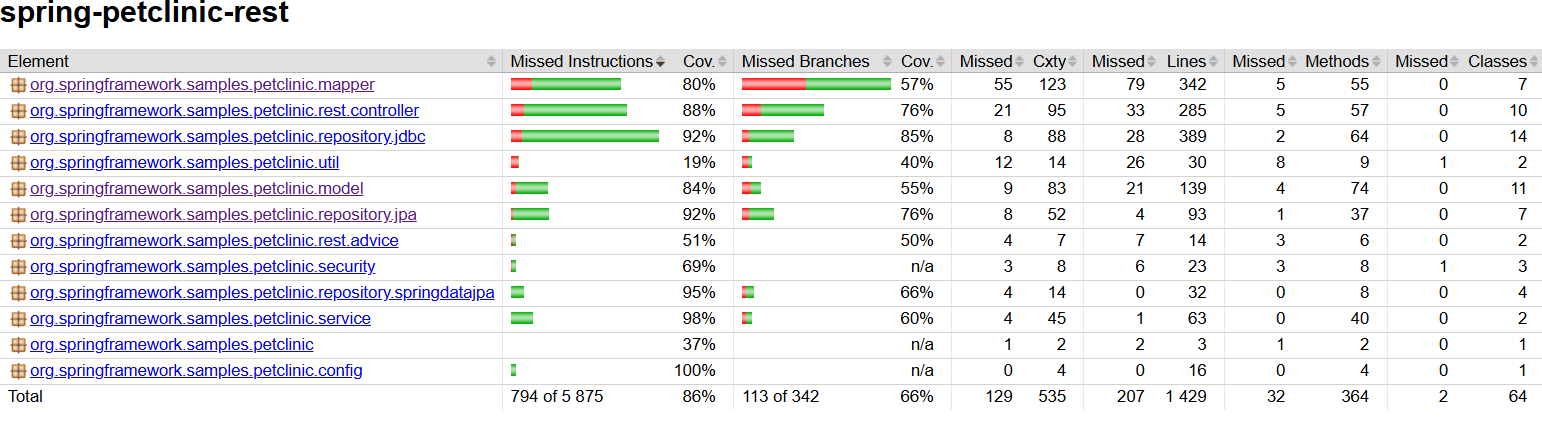
\includegraphics[width=\textwidth]{figs/Funcional Correctness/overall report.png}
			\caption{Overall Coverage}
			\label{fig:Overall Report}
		\end{figure}
		\vspace{1em}
		
		The overall code coverage results indicate that 86\%  of the project's instructions are covered by tests, reflecting a solid testing foundation. The config package achieves perfect coverage at 100\%, while the util package has the lowest at 19\%. For branch coverage, the project scores 66\% overall, with the repository.jdbc package leading at 85\%. However, the model package shows lower branch coverage, suggesting untested logical paths within those classes. The services package, which handles complex operations, demonstrates strong test coverage, emphasizing its importance in the project.
		
		
		
		
		\section{PetType Code Coverage}
		In this section, I will verify and analyze the code coverage of the PetType class. In order to do that, I will focus on the packages that contain the functionalities of the Pet Clinic and the Pets. Those package are:
		\begin{itemize}
			\item Mapper
			\item Rest Controller
			\item Model
		\end{itemize} 
		
		
		
		\newpage
		\subsection{Mapper}
		\begin{figure}[H]
			\centering
			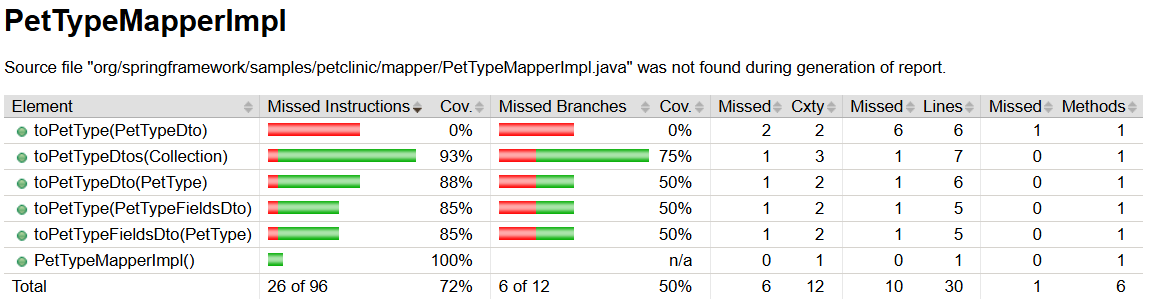
\includegraphics[width=\textwidth]{figs/Funcional Correctness/PetTypeMapperImpl.png}
			\caption{PetTypeMapperImpl Coverage}
			\label{fig:PetTypeMapperImpl}
		\end{figure}
		
		After examining the JaCoCo analysis of PetTypeMapperImpl, Figure \ref{fig:PetTypeMapperImpl}, we see the 72\% coverage and 50\% branch coverage, indicating that, even though the majority of the code is being tested, there is still a significant portion of code that remains untested, which could potentially affect the reliability of the application
		The methods toPetTypeDtos(Collection), toPetTypeDto(PetType), toPetType(PetTypeFieldsDto), and toPetTypeFieldsDto(PetType) have code coverages of 93\%, 88\%, 85\%, and 85\%, respectively, indicating that these methods are generally well-tested, though there may still be some areas for improvement to ensure comprehensive test coverage.
		Notably, the method toPetType(PetTypeDto) has 0\% coverage, highlighting an area for improvement to enhance application reliability.
		
		
		
		\subsection{Rest Controller}
		\begin{figure}[H]
			\centering
			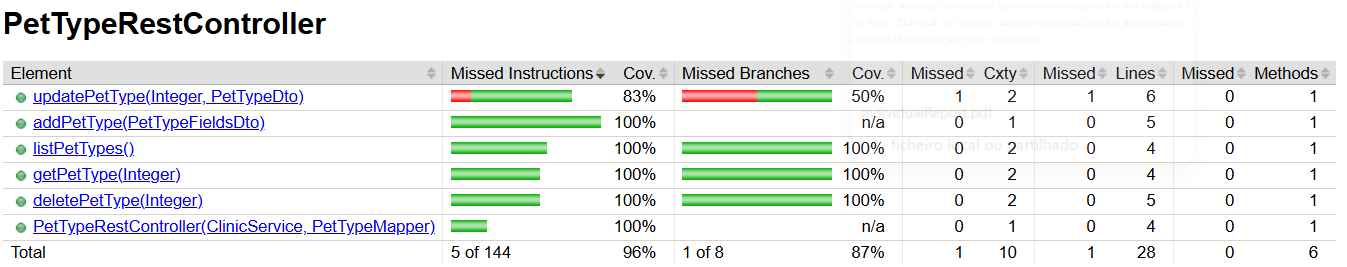
\includegraphics[width=\textwidth]{figs/Funcional Correctness/PetTypeRestController.png}
			\caption{PetTypeModel Coverage}
			\label{fig:PetTypeRestController}
		\end{figure}
		After examining the JaCoCo analysis of PetTypeRestController, Figure \ref{fig:PetTypeRestController}, we can see that the coverage is 96\% and the branch coverage is 87\%, indicating a strong testing foundation for the class. However, the branch coverage suggests that there is still one untested branch, which could lead to potential issues in specific scenarios.
		
		
		
		\subsection{Model}
		\begin{figure}[H]
			\centering
			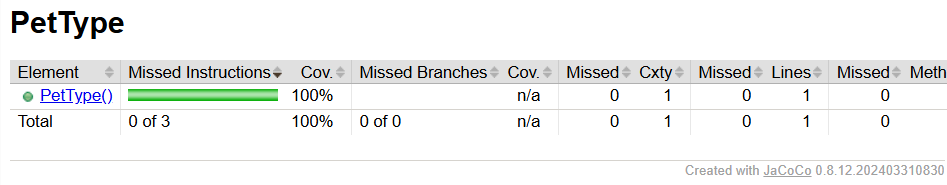
\includegraphics[width=\textwidth]{figs/Funcional Correctness/PetTypeModel.png}
			\caption{PetTypeModel Coverage}
			\label{fig:PetTypeModel}
		\end{figure}
		After examining the JaCoCo analysis of PetTypeModel, Figure \ref{fig:PetTypeModel}, we can see that coverage analysis of the PetType model reveals an impressive 100\% coverage rate, indicating that all instructions are tested. However, it is important to note that the model is relatively small, consisting of only three instructions. While the high coverage is good, the limited size of the model suggests that the coverage metric should be interpreted with caution.
		
		
		\section{Flaky Tests}
		
			Flaky tests are tests that sometimes pass and sometimes fail without any changes to the codebase, test logic, or environment. This inconsistency makes them unreliable and difficult to trust, as they can obscure real issues or cause false alarms. Therefore, the presence of flaky tests indicates a problem in the way the tests are constructed, making it essential to identify and resolve the root cause.

		To help detect flaky tests, we will use the flaky-test-extractor-maven-plugin, which has been added to the pom.xml.


		\begin{figure}[H]
		  \centering
		  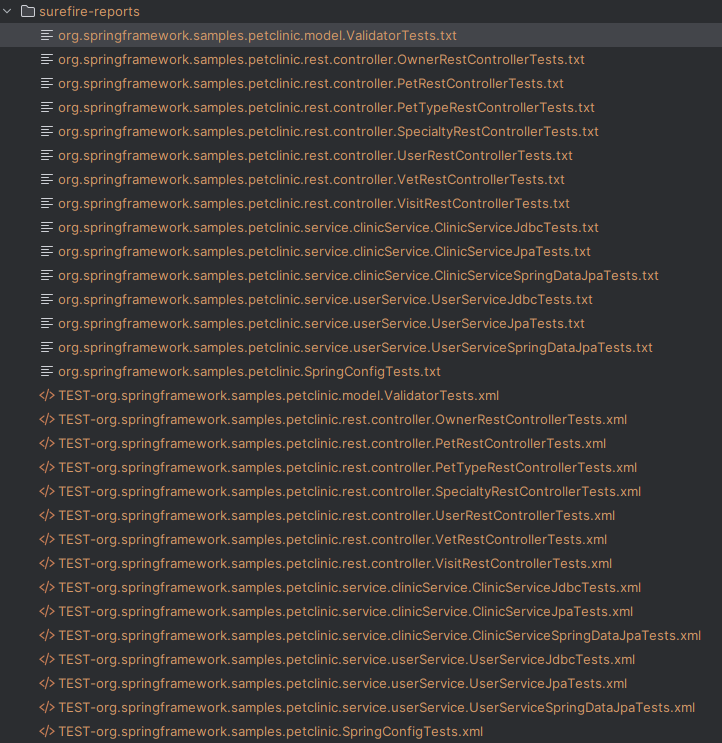
\includegraphics[width=0.7\textwidth]{figs/Funcional Correctness/FlakyTestsReport.png}
		  \caption{Flaky Tests Report}
		  \label{fig:FlakyTestsReport}
		\end{figure}

	Based on the report in Figure \ref{fig:FlakyTestsReport} we can see that no file has the suffix -FLAKY, indicating that there are no flaky tests in this project.
	%% =================================	
	\chapter{Maintainability}
\textit{Maintainability is the measure of how easily a software system can be altered after its initial deployment. Good maintainability affects how effortlessly a system can be updated, improved, or fixed to address new requirements, correct issues, or enhance performance. In this analysis, Sonargraph Explorer will be used to assess the relevant metrics in the subsequent sections. }
	

\section{Coupling and Structural Erosion}

\textbf{Metric:} Average Component Dependency (ACD) \\
\textbf{Category:} Cohesion/Coupling (John Lakos) \\
\textbf{Value:} 7.66

The ACD value of 7.66 indicates that, on average, each component in the system depends on approximately 7-8 other components, both directly and indirectly. This level of dependency suggests a moderate degree of coupling among components. While the architecture is modular enough to allow individual components to function, this level of coupling may require careful attention when refactoring or updating components to prevent unintended interactions.

A high ACD value could signal challenges in maintaining and evolving the code, as each component's dependencies may limit its flexibility and increase the likelihood of cascading changes. Reducing dependencies where possible can improve modularity and ease of maintenance.

\begin{figure}[H]
	\centering
	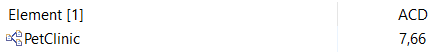
\includegraphics[width=0.7\textwidth]{figs/Maintainability/ACD.png}
	\caption{ACD Metric}
	\label{fig:ACD}
  \end{figure}

\section{Size and Complexity}

\textbf{Metric:} Number of Components/Sources \\
\textbf{Category:} Size \\
\textbf{Value:} 131

The project consists of 131 components or source files, which provides a structural overview of its size and organization. In the context of a codebase with close 10000 lines of code, the distribution of 131 components suggests an average of approximately 74 lines per component. This number points to a relatively well-organized project structure, where code is compartmentalized across manageable components, aiding readability, traceability, and modularity. This organizational structure can support ongoing maintainability by making individual components easier to understand, modify, and test.

\begin{figure}[H]
	\centering
	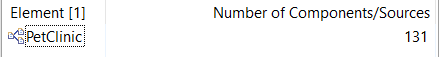
\includegraphics[width=0.7\textwidth]{figs/Maintainability/NumberOfComponent-Sources.png}
	\caption{Number Of Component and Sources Metric}
	\label{fig:NumberOfComponent-Sources}
  \end{figure}




\section{Cyclomatic Complexity to three methods}
The cyclomatic complexity of a code section is the quantitative measure of the number of linearly independent paths in it. It is a software metric used to indicate the complexity of a program. 

To calculate the cyclomatic complexity we use:
\begin{itemize}
	\item \textbf{CC = D + 1}
	\item D = the number loop statement or conditional statement (Decision Points) 

\end{itemize}

Now I will calculate the Cyclomatic Complexity of the following methods


\textbf{getPetType}


In the method \ref{fig:getPetType}, there is one decision point (the conditional statement if (petType == null)). This conditional statement divides the flow into two paths, and therefore, the Cyclomatic Complexity is:

\textbf{CC = D + 1 = 1 + 1 = 2}
\begin{figure}[H]
	\centering
	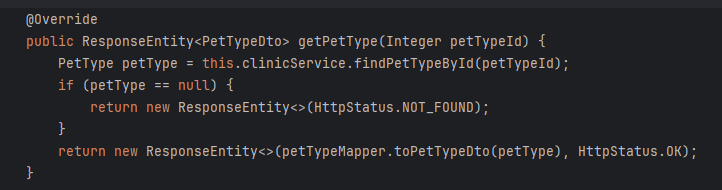
\includegraphics[width=\textwidth]{figs/Maintainability/getPetType.png}
	\caption{getPetType Method}
	\label{fig:getPetType}
  \end{figure}

\textbf{updatePetType}


In the method \ref{fig:updatePetType}, there is one decision point (the conditional statement if (currentPetType == null)). This conditional statement splits the flow into two possible paths. Therefore, the Cyclomatic Complexity is:
\textbf{CC = D + 1 = 1 + 1 = 2}
\begin{figure}[H]
	\centering
	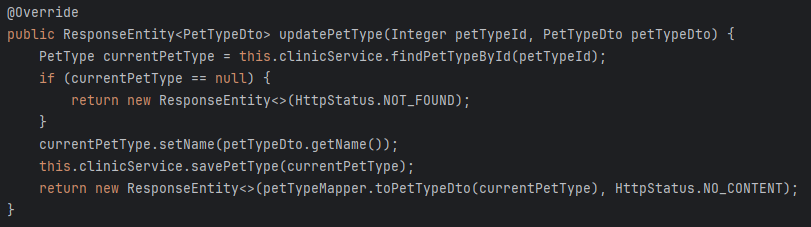
\includegraphics[width=0.7\textwidth]{figs/Maintainability/updatePetType.png}
	\caption{updatePetType Method}
	\label{fig:updatePetType}
  \end{figure}

\textbf{deletePetType}


In the method \ref{deletePetType}, there is one decision point (the conditional statement if (currentPetType == null)). This conditional statement splits the flow into two possible paths. Therefore, the Cyclomatic Complexity is:
\textbf{CC = D + 1 = 1 + 1 = 2}
\begin{figure}[H]
	\centering
	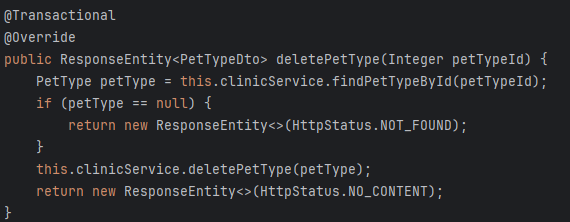
\includegraphics[width=0.7\textwidth]{figs/Maintainability/deletePetType.png}
	\caption{deletePetType Method}
	\label{fig:deletePetType}
  \end{figure}



  Based on the results, we can see that all three methods have a Cyclomatic Complexity of 2, indicating a low level of complexity with only one decision point. This suggests that the methods are straightforward and require two test cases to fully cover both execution paths.


  \section{Instability}

Instability measures a class's dependency on other classes and how much other classes depend on it. A high instability value indicates a class with many dependencies, while a low value suggests a more independent and stable class.

In order to calculate the Instability of the class we will use the following formula
\begin{itemize}
	\item Instability = E / (I + E)
	\item E is the number of outgoing dependencies (Efferent Coupling).
	\item I is the number of incoming dependencies (Afferent Coupling).
\end{itemize}
We will calculate the Instability of the module PetType.java 

\begin{figure}[H]
	\centering
	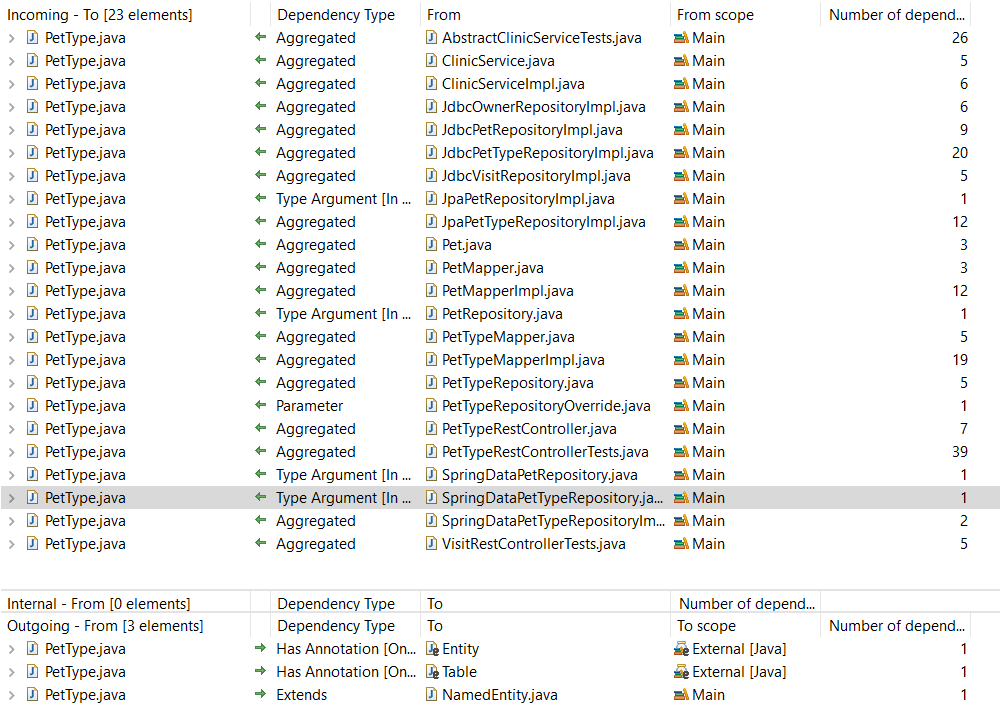
\includegraphics[width=0.7\textwidth]{figs/Maintainability/DependenciesPetType.png}
	\caption{Dependencies PetType}
	\label{fig:DependenciesPetType}
  \end{figure}

\textbf{Efferent Coupling (E) and Afferent Coupling(I)}


As seen in the figure \ref{fig:DependenciesPetType} the module PetType has a total of 3 outgoing dependencies. On the other hand we have a significant amount of Incoming dependencies with 23 elements. 

Using the formula that we expecified earlier we get

\textbf{Instability = 3 / (3 + 23) = 3 / 26 = 0.11}

An instability value of 0.11 indicates that the class is relatively stable, with few dependencies on other classes and minimal impact when changes occur in external components. This suggests that the class is well-contained and less prone to breakage during maintenance, which is generally a positive characteristic for maintainability.



\section{Maintainability of test code}
Now I will explore and examine testing smells in this project. Test smells refer to possible violations of best practices in testing code, that can compromise the reliability and effectiveness of tests. Eventhough they are sometimes ignored, testing smells can lead to false positives or negatives and make tests harder to maintain or comprehend

\begin{figure}[H]
	\centering
	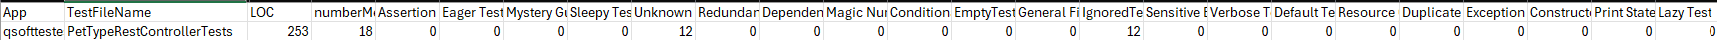
\includegraphics[width=\textwidth]{figs/Maintainability/TestSmells.png}
	\caption{TestSmells PetType}
	\label{fig:TestSmells}
  \end{figure}

  As shown in Figure \ref{fig:TestSmells}, we analyzed 18 test methods. Out of these, 12 were initially labeled as "Unknown tests" and later classified as "IgnoredTests." This means that only six tests passed the jNose test smells criteria, indicating a deficiency in the project's testing quality that should be addressed and improved.







	%% =================================		
	\chapter{Performance}
In software development, the performance of an application is crucial for its success and integration within a larger system. The efficiency and responsiveness of an application greatly influence the user experience and overall user satisfaction. This evaluation focuses on analyzing the performance aspects of the current project. Performance analysis is essential as it reveals the application’s ability to handle different workloads, respond quickly to user interactions, and utilize resources optimally.

To conduct a thorough performance assessment, I will use JMeter and K6, both powerful testing tools renowned for their ability to evaluate the performance of software applications. JMeter will simulate various scenarios that mimic real-world usage conditions, while K6 will be used to performe the same exact performance tests, collecting valuable data to assess the project’s performance characteristics.

In the following sections, we will explore specific performance metrics, analyze the results obtained from JMeter and K6 tests, and draw conclusions about the project’s suitability for integration into a larger system based on its performance attributes.

  \section{Requirements}

In order to have a standard, we consider that, for normal conditions, the application
must:


\textbf{In normal conditions:}
		\begin{itemize}
			\item Respond to any type of request in less than 3 seconds 99\% of the time;
			\item Process more than 250 requests per second.
		\end{itemize}
		
	\textbf{In heavy conditions:}
		\begin{itemize}
			\item Supports heavy user access of up to 200 users;
			\item Process more than 150 requests per second.
		\end{itemize}


  \section{Testing Environment}
  All tests conducted for this evaluation were performed on a single machine/computer, with the specifications outlined in the image below (\ref{fig:SystemDetails}). It's important to note that the computer remained consistently connected to the internet via an Ethernet cable throughout the testing process. This ensures a consistent and standardized testing environment, allowing for accurate and reliable performance assessments under the specified configurations. The use of a wired connection guarantees stable network conditions, contributing to the precision of the results obtained during the evaluation.
  
  	\begin{figure}[h]
    	\centering
    	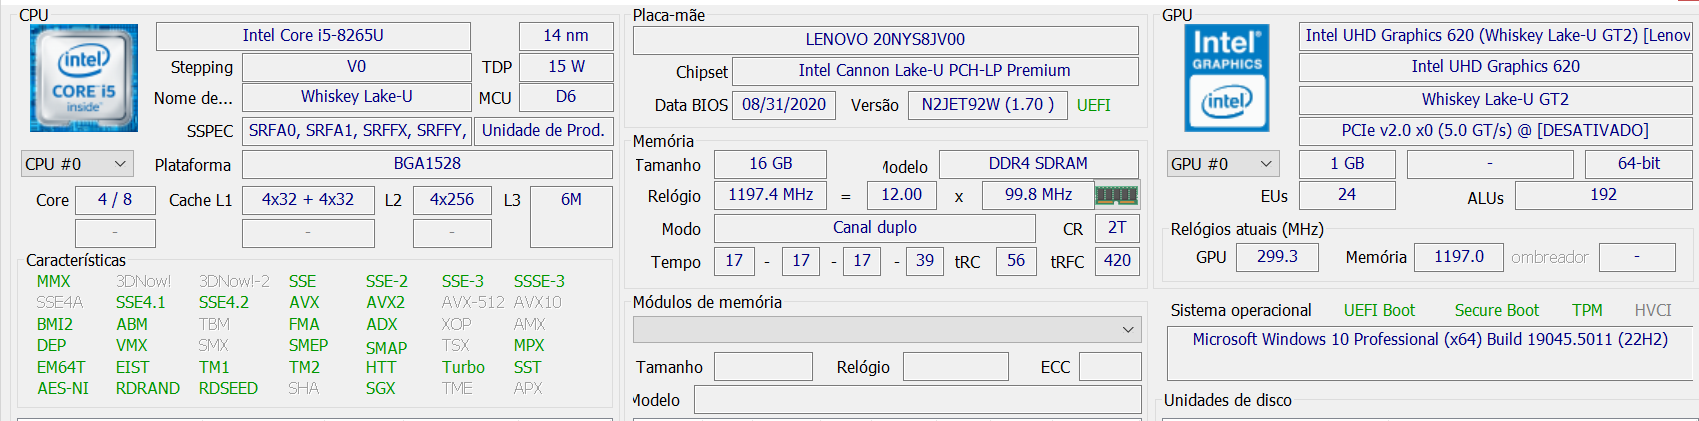
\includegraphics[width=\textwidth]{figs/Performance/SystemDetails.png}
    	\caption{System Details}
    	\label{fig:SystemDetails}
  	\end{figure}

\section{Load Test}
		
		Load testing evaluates a system's behavior under typical conditions by simulating realistic user activity. This process enables the early identification of performance issues, such as response time delays and resource overuse, even at normal load levels. Additionally, it provides insights into the system’s capacity, supporting scalability planning to ensure it can handle anticipated user growth effectively.
		In this section we will evaluate the Loads tests to the endpoints GET and POST of petType
		\subsection{Scenario GET}
		\begin{itemize}
			\item 50 users of the web application;
	           \item Requesting all existing PetTypes
			\item The system returns a list with all PetTypes
			\item Less than 3 seconds 99\% of the times;
			\item Normal Load.
		\end{itemize}


		\subsection{Jmeter}


		\textbf{Test Configuration}

		\begin{figure}[H]
			\centering
			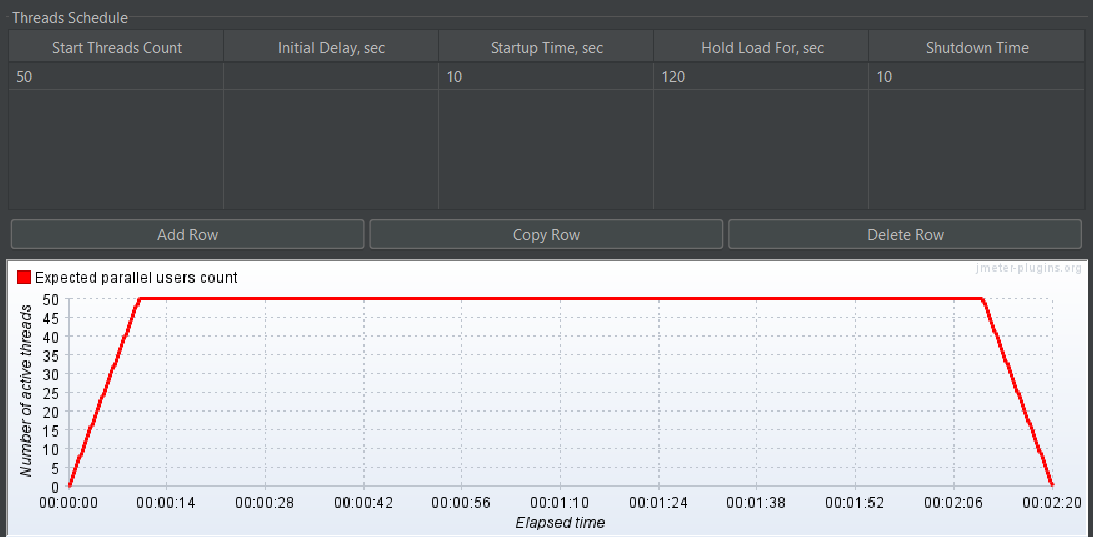
\includegraphics[width=0.7\textwidth]{figs/Performance/Test Configuration/JMETER-LOAD.png}
			\caption{Jmeter Load Configuration}
			\label{fig:JMETER-LOAD}
		\end{figure}

		\begin{figure}[H]
			\centering
			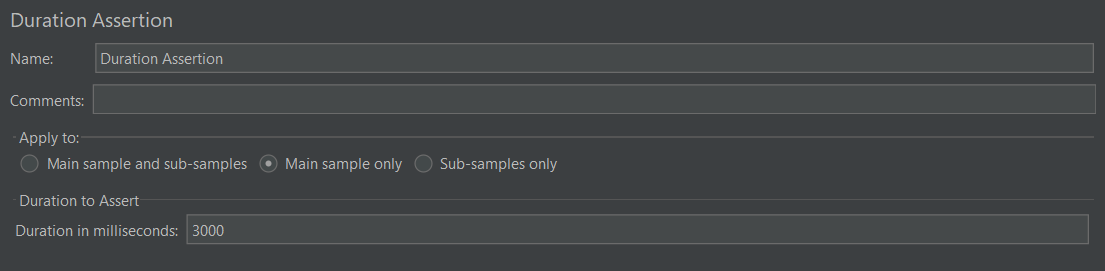
\includegraphics[width=0.7\textwidth]{figs/Performance/Test Configuration/Duration-SOAK-LOAD-JMETER.png}
			\caption{Duration GET Load Configuration}
			\label{fig:DurationGetLoad}
		\end{figure}

		Based on the scenario we designed earlier I created the Jmeter Load Configuration that holds for 120 seconds 50 Threads (Users), as seen in the Figure \ref{fig:JMETER-LOAD}. In the Figure \ref{fig:DurationGetLoad} I've set the maximum duration to 3000 milliseconds.



		\textbf{Results}


		\begin{figure}[H]
			\centering
			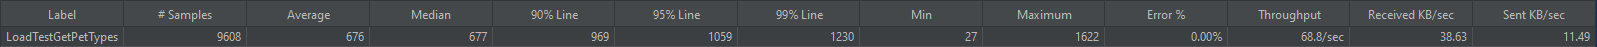
\includegraphics[width=\textwidth]{figs/Performance/Results/JMETER GET LOAD AR.png}
			\caption{GET Load Test Aggregate Report}
			\label{fig:GETLoadAggregateReport}
		\end{figure}
		\begin{figure}[H]
			\centering
			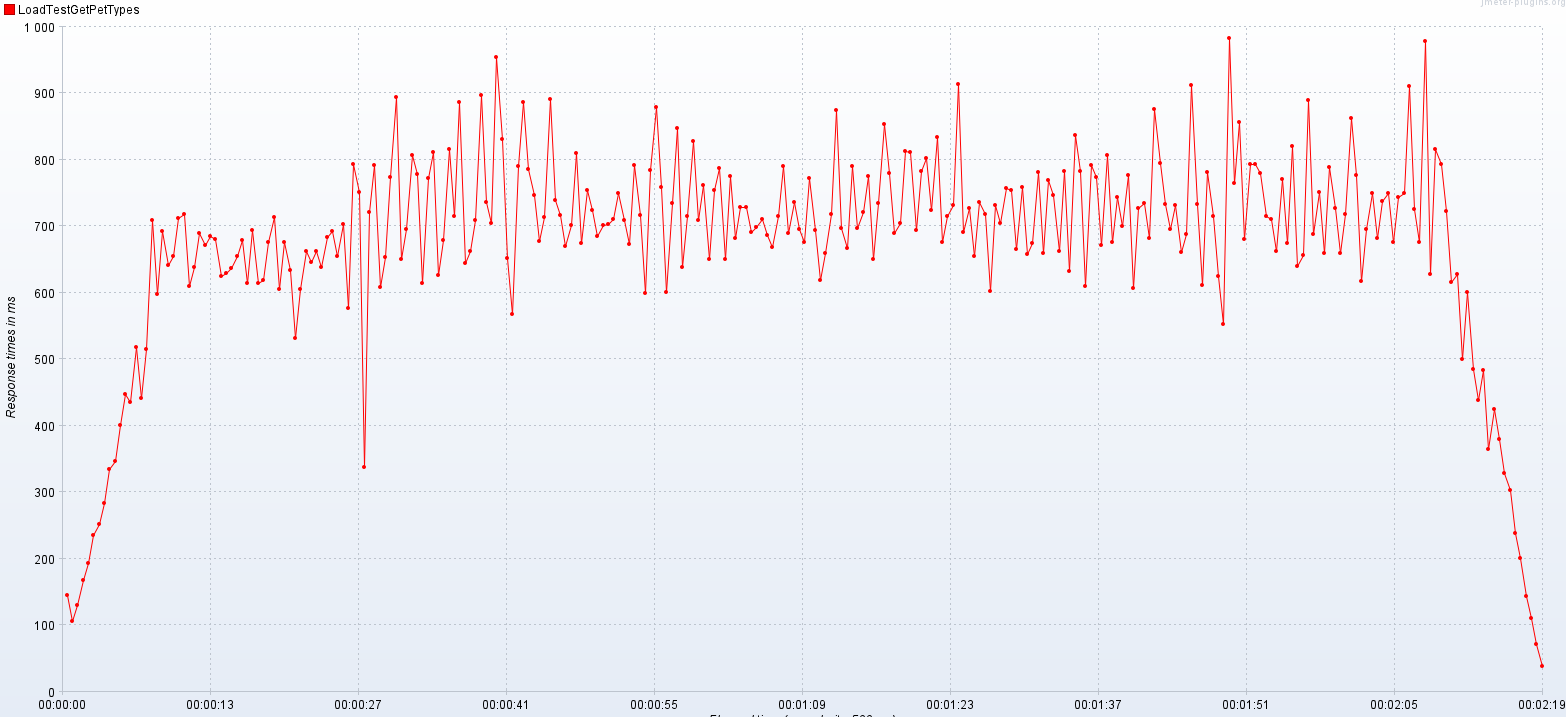
\includegraphics[width=0.7\textwidth]{figs/Performance/Results/JMETER GET LOAD ROT.png}
			\caption{GET Load Test Responses Over Time}
			\label{fig:GETLoadResposesOverTime}
		\end{figure}

		The results, seen in Figure \ref{fig:GETLoadAggregateReport}, indicate that the API performs incredibly well under this scenario, with 0\% errors and an average response time of 676 ms. The highest response time was just 1622 ms, which equates to half of the maximum defined.
		In Figure \ref{fig:GETLoadResposesOverTime}, we can see the response times over time, which remained stable throughout the entire process		
		\subsection{K6}


		\textbf{Test Configuration}
		\begin{figure}[H]
			\centering
			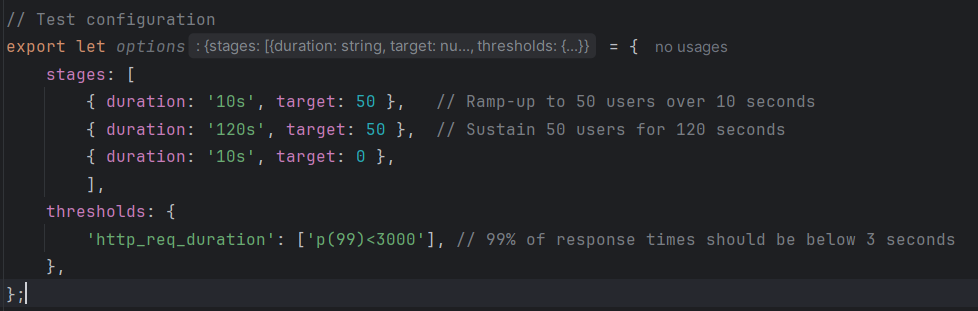
\includegraphics[width=0.7\textwidth]{figs/Performance/Test Configuration/K6-LOAD.png}
			\caption{K6 Load Configuration}
			\label{fig:K6-LOAD}
		\end{figure}
		Similar to the JMeter configuration, in the k6 test, I configured the test to hold 50 users for 120 seconds, as shown in Figure \ref{fig:K6-LOAD}. I've also set the Duration to be less than 3000 milliseconds.
		

		\textbf{Results}
		\begin{figure}[H]
			\centering
			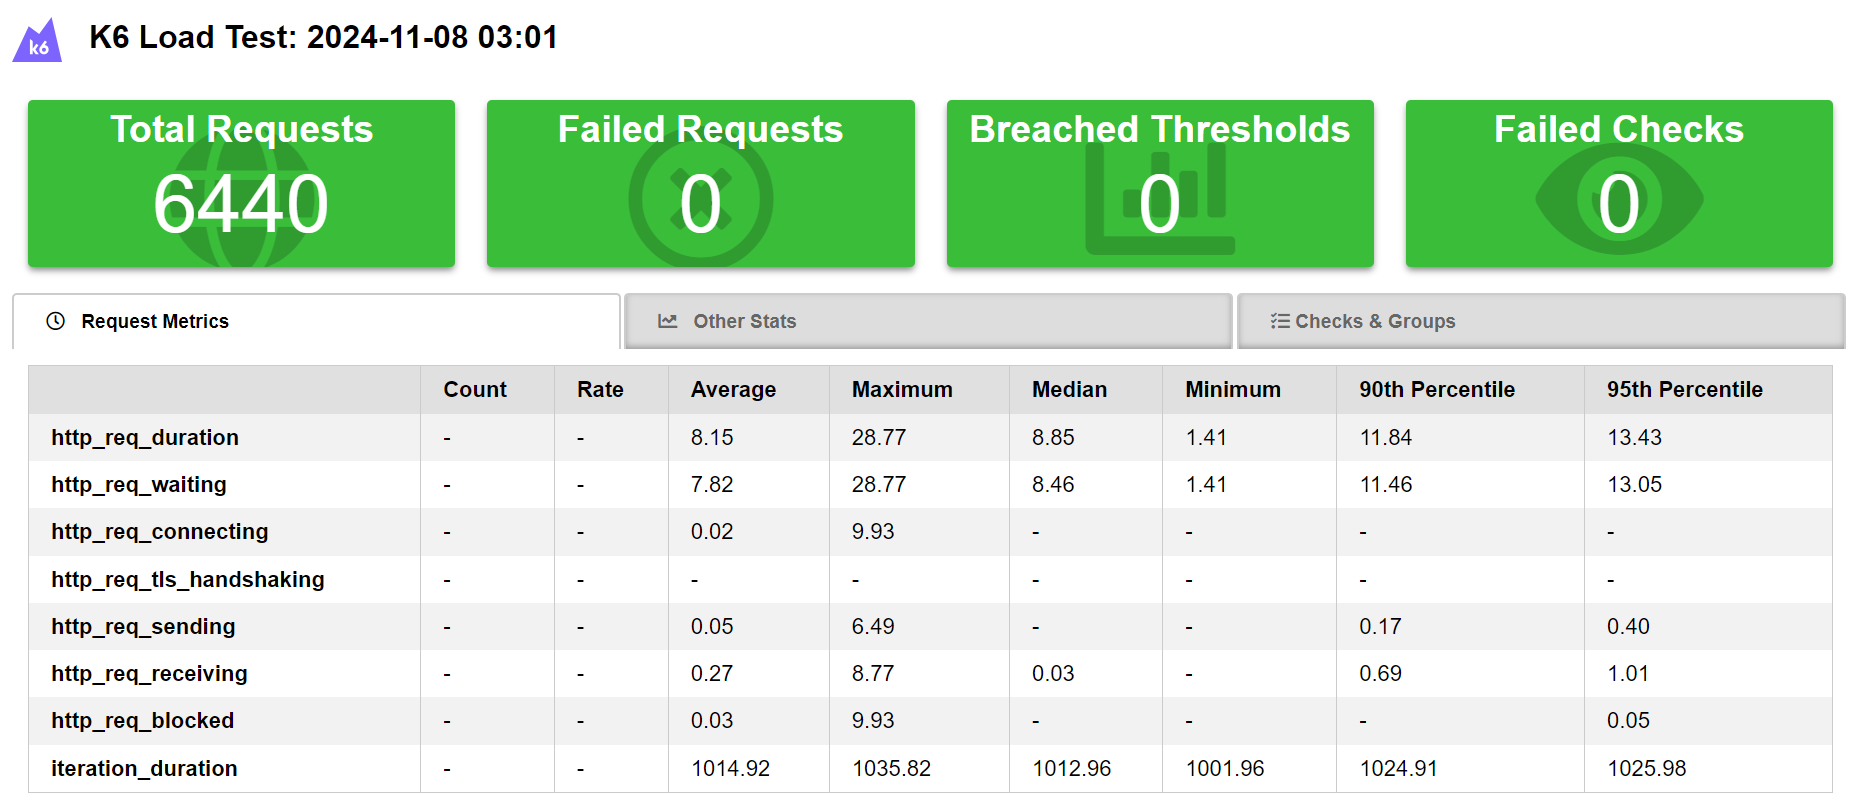
\includegraphics[width=0.7\textwidth]{figs/Performance/Results/K6 GET LOAD.png}
			\caption{K6 GET LOAD}
			\label{fig:K6-GET-LOAD}
		\end{figure}
		The results, seen in Figure \ref{fig:K6-GET-LOAD}, indicate that the API performs incredibly well under this scenario, with 0 failed request and an average response time of just 1014 ms. The highest response time was just 1035 ms, which is lower than the maximum defined.

		\subsection{Scenario POST}
		\begin{itemize}
			\item 50 users of the web application;
	        \item Posting a new PetTypes
			\item The system returns 201
			\item Less than 3 seconds 99\% of the times;
			\item Normal Load.
		\end{itemize}

		\subsection{Jmeter}

		\textbf{Load CSV}
		\begin{figure}[H]
			\centering
			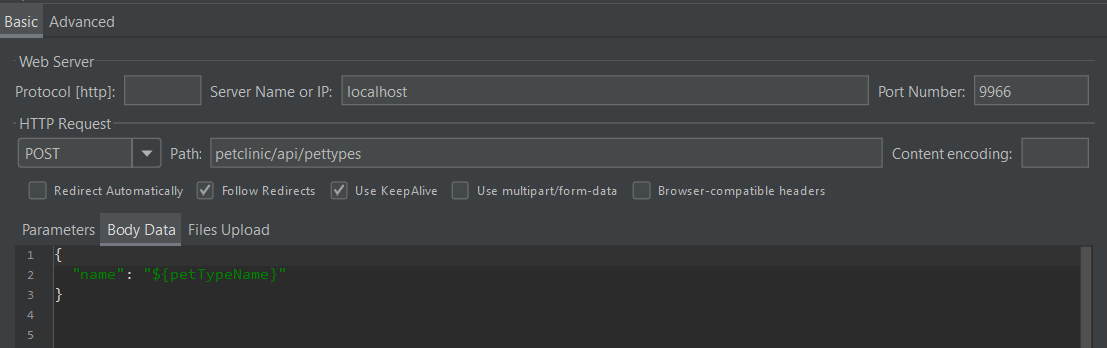
\includegraphics[width=0.7\textwidth]{figs/Performance/Test Configuration/LoadCSV-Jmeter.png}
			\caption{LoadCSV Jmeter}
			\label{fig:LoadCSV Jmeter}
		 \end{figure}
		\begin{figure}[H]
			\centering
			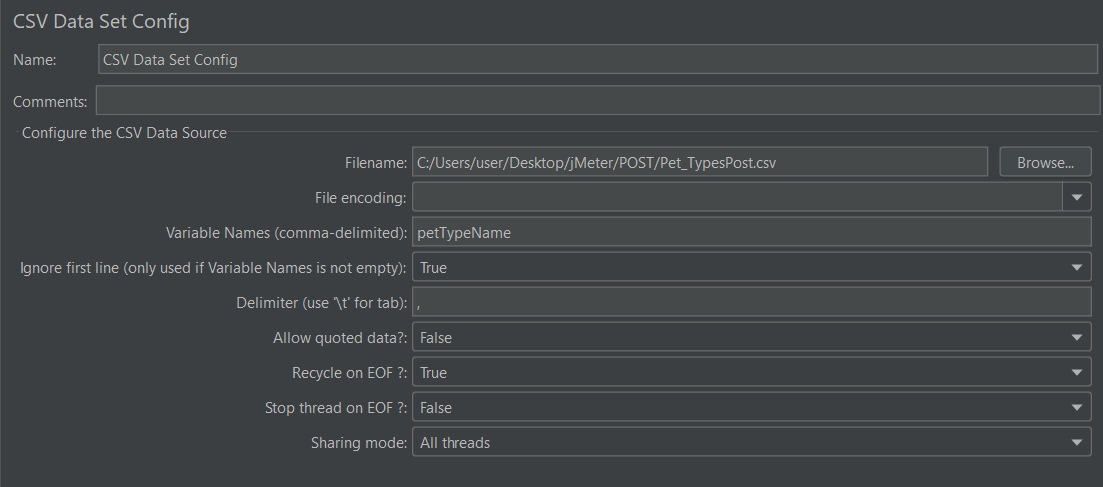
\includegraphics[width=0.7\textwidth]{figs/Performance/Test Configuration/LoadCSV-Jmeter2.png}
			\caption{LoadCSV Jmeter2}
			\label{fig:LoadCSV Jmeter2}
		 \end{figure}

		 In the figure \ref{fig:LoadCSV Jmeter2} we can see the configuration needed in jmeter in order to use an CSV Data Set for the tests. In the figure \ref{fig:LoadCSV Jmeter} we can see the body Data in order to use the csv data.


		\textbf{Test Configuration}
		\begin{figure}[H]
			\centering
			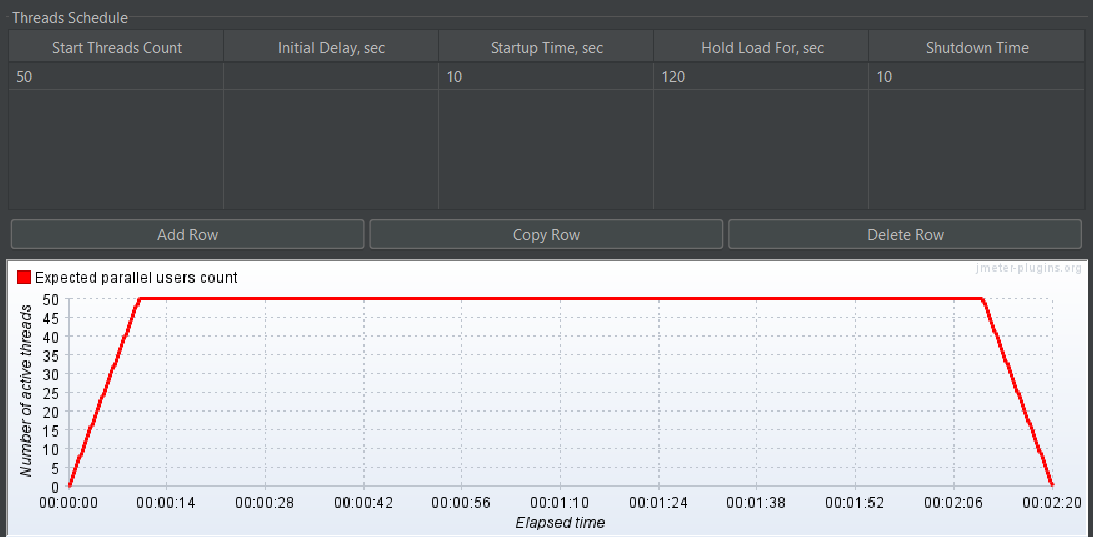
\includegraphics[width=0.7\textwidth]{figs/Performance/Test Configuration/JMETER-LOAD.png}
			\caption{Jmeter Load Configuration}
			\label{fig:JMETER-LOADPOST}
		\end{figure}
		\begin{figure}[H]
			\centering
			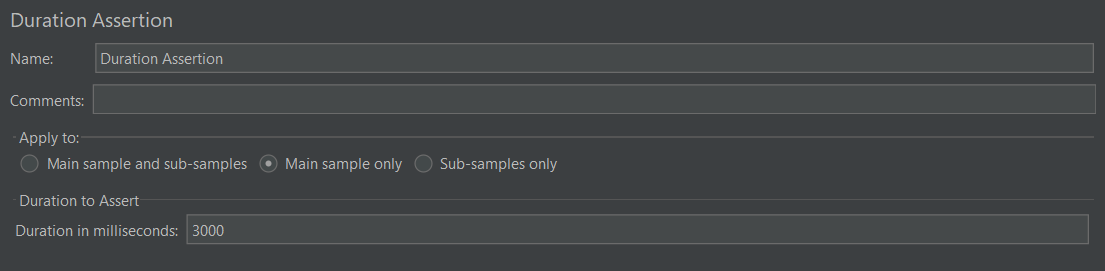
\includegraphics[width=0.7\textwidth]{figs/Performance/Test Configuration/Duration-SOAK-LOAD-JMETER.png}
			\caption{Duration POST Load Configuration}
			\label{fig:DurationPostLoad}
		\end{figure}


		Based on the scenario we designed earlier I created the Jmeter Load Configuration that holds for 120 seconds 50 Threads (Users), as seen in the Figure \ref{fig:JMETER-LOADPOST}. In the Figure \ref{fig:DurationPostLoad} I've set the maximum duration to 3000 milliseconds.



		\textbf{Results}
		\begin{figure}[H]
			\centering
			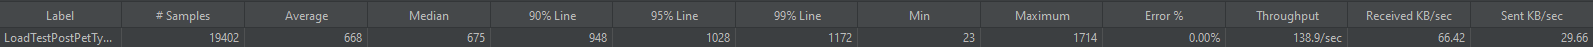
\includegraphics[width=\textwidth]{figs/Performance/Results/JMETER POST LOAD AR.png}
			\caption{POST Load Test Aggregate Report}
			\label{fig:PostLoadAggregateReport}
		\end{figure}
		\begin{figure}[H]
			\centering
			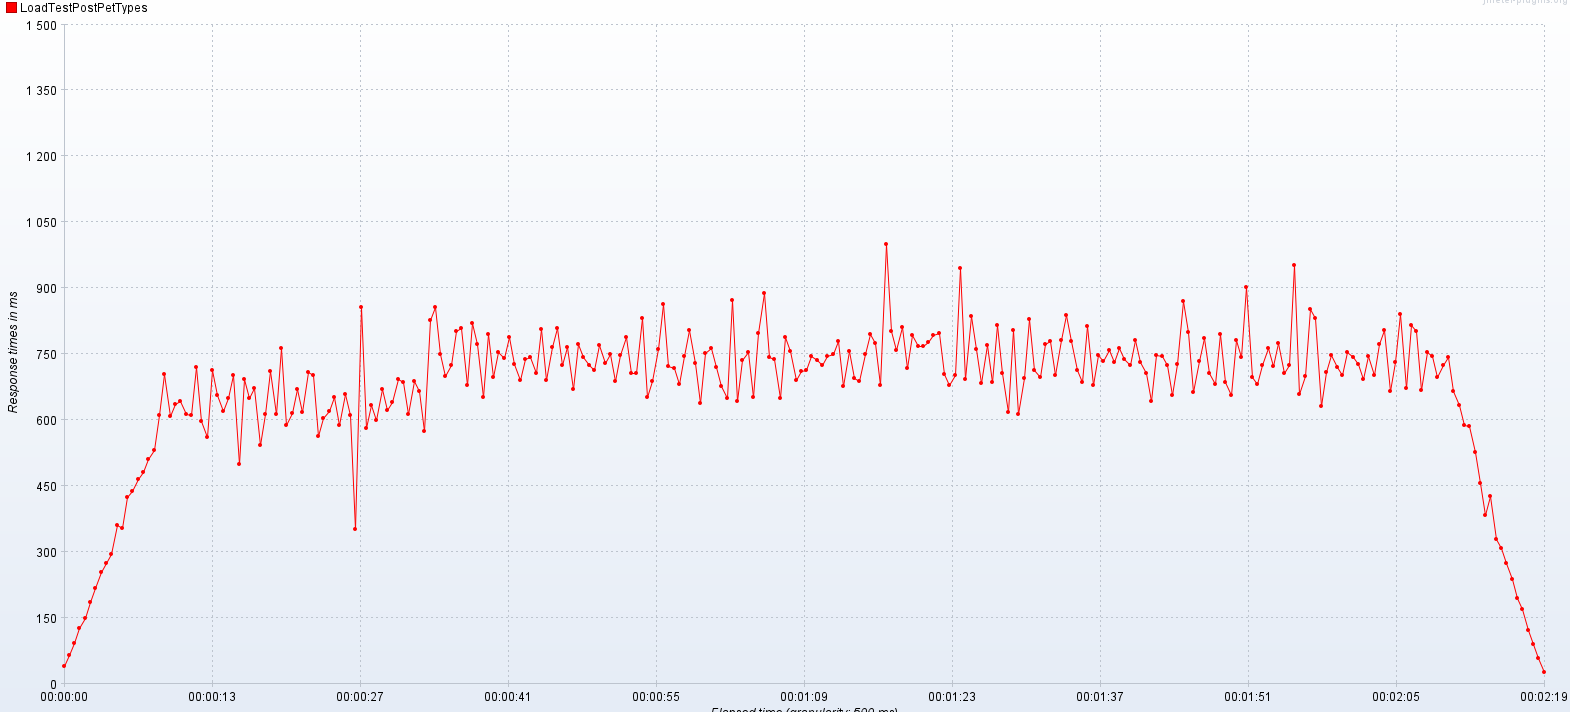
\includegraphics[width=0.7\textwidth]{figs/Performance/Results/JMETER POST LOAD ROT.png}
			\caption{GET Post Test Responses Over Time}
			\label{fig:GETPostResposesOverTime}
		\end{figure}
		The results, seen in Figure \ref{fig:PostLoadAggregateReport}, indicate that the API performs incredibly well under this scenario, with 0\% errors and an average response time of 668 ms. The highest response time was just 1714 ms, which is a little bit over the half of the maximum defined.
		In Figure \ref{fig:GETPostResposesOverTime}, we can see the response times over time, which remained stable throughout the entire process		


		\subsection{K6}

		\textbf{Load CSV}
		\begin{figure}[H]
			\centering
			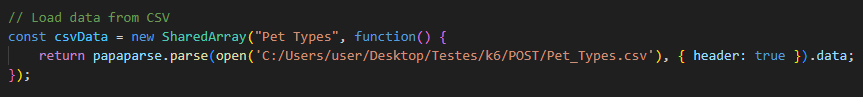
\includegraphics[width=0.7\textwidth]{figs/Performance/Test Configuration/LoadCSV-K6.png}
			\caption{LoadCSV K6}
			\label{fig:LoadCSV K6}
		\end{figure}
		In the figure \ref{fig:LoadCSV K6} we can see the configuration needed in K6 in order to use an CSV Data Set for the tests.


		\textbf{Test Configuration}
		\begin{figure}[H]
			\centering
			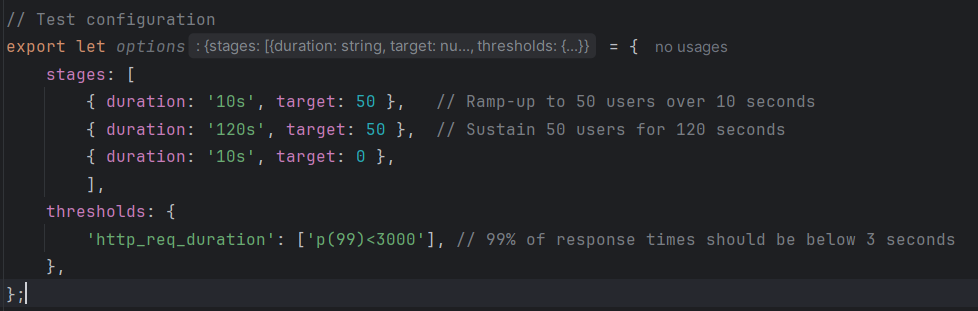
\includegraphics[width=0.7\textwidth]{figs/Performance/Test Configuration/K6-LOAD.png}
			\caption{K6 Load Configuration}
			\label{fig:K6-LOAD-POST}
		\end{figure}
		Similar to the JMeter configuration, in the k6 test, I configured the test to hold 50 users for 120 seconds, as shown in Figure \ref{fig:K6-LOAD-POST}. I've also set the Duration to be less than 3000 milliseconds.

		\textbf{Results}
		\begin{figure}[H]
			\centering
			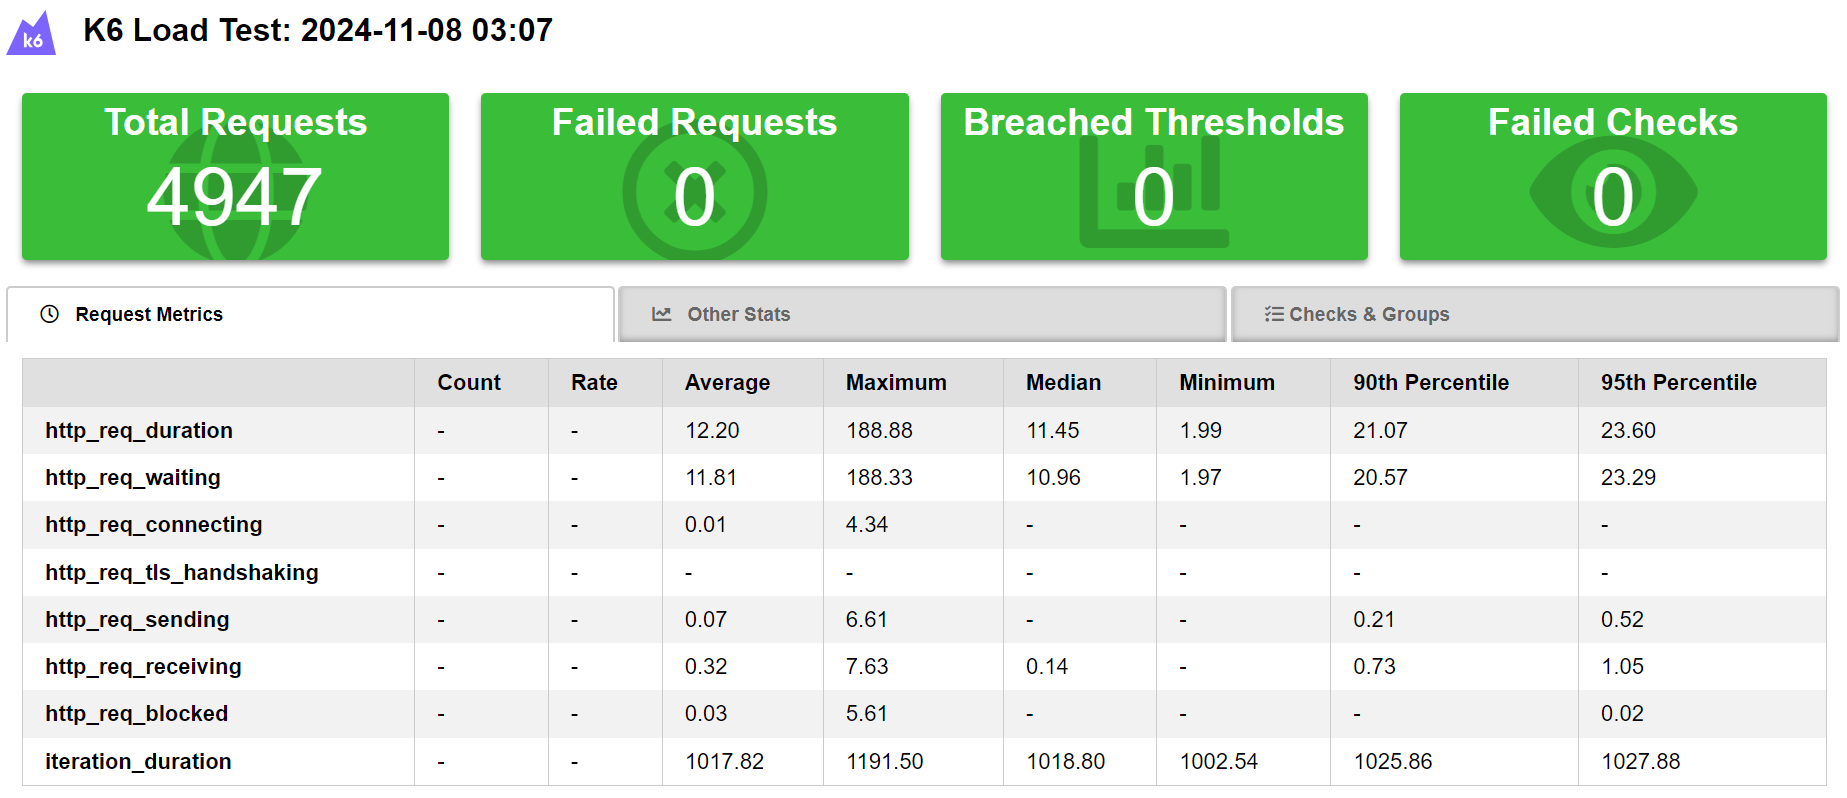
\includegraphics[width=0.7\textwidth]{figs/Performance/Results/K6 POST LOAD.png}
			\caption{K6 POST LOAD}
			\label{fig:K6-POST-LOAD}
		\end{figure}
		The results, seen in Figure \ref{fig:K6-POST-LOAD}, indicate that the API performs incredibly well under this scenario, with 0 failed request and an average response time of just 1017 ms. The highest response time was just 1191 ms, which is lower than the maximum defined.

\section{Stress Test}
		
	Stress testing involves subjecting the system to conditions that exceed its standard operational limits to assess its behavior under severe strain. This type of testing facilitates
crucial insights, including resilience evaluation, which examines the system’s capacity
to recover from high-stress situations and whether it maintains functionality or fails
catastrophically. Furthermore, it assists in identifying the failure threshold, providing
an understanding of the system’s limits and its response under extreme conditions.
		
		\subsection{Scenario GET}
		\begin{itemize}
			\item 200 users of the web application;
			\item Requesting all existing PetTypes
			\item The system returns a list with all PetTypes
			\item Less than 3 seconds 99\% of the times;
			\item Heavy Load.
		\end{itemize}

		\subsection{Jmeter}
		\textbf{Test Configuration}
		\begin{figure}[H]
			\centering
			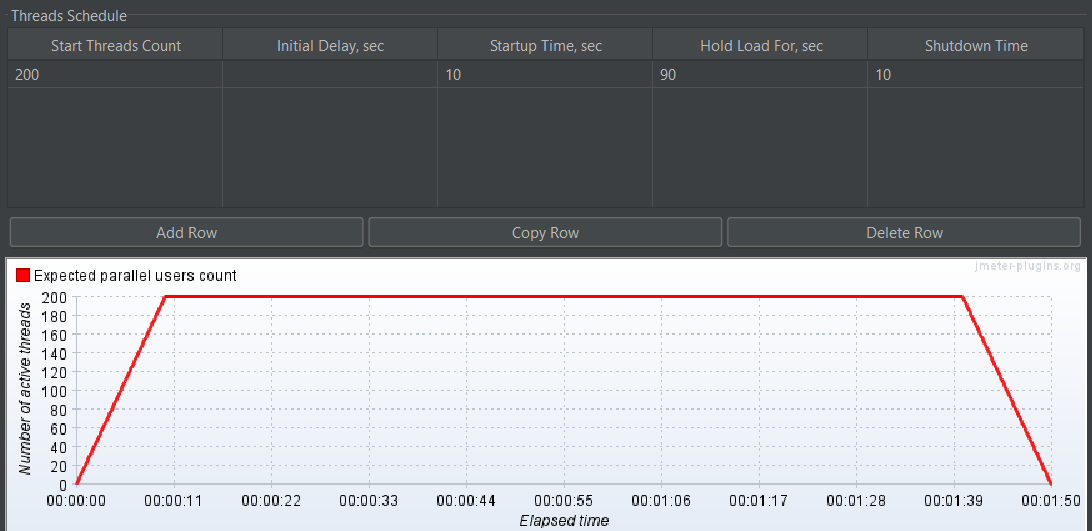
\includegraphics[width=0.7\textwidth]{figs/Performance/Test Configuration/JMETER-STRESS.png}
			\caption{Jmeter Stress Configuration}
			\label{fig:JMETER-STRESS}
		\end{figure}
		\begin{figure}[H]
			\centering
			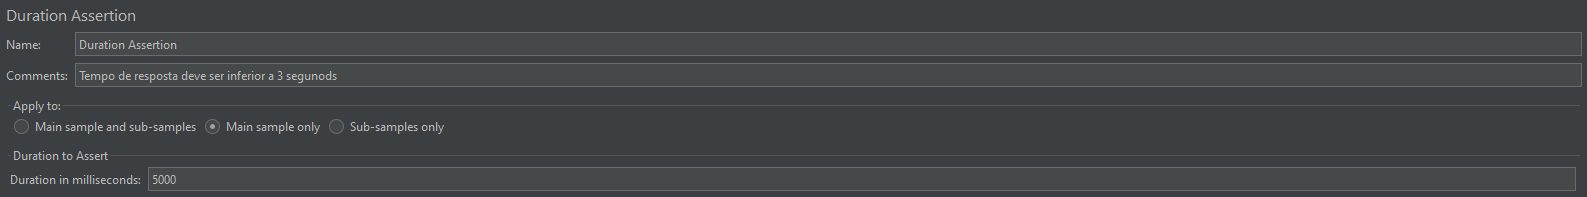
\includegraphics[width=0.7\textwidth]{figs/Performance/Test Configuration/Duration-Stress.png}
			\caption{Duration GET Stress Configuration}
			\label{fig:DurationGetStress}
		\end{figure}

		Based on the scenario we designed earlier I created the Jmeter Stress Configuration that holds for 90 seconds 200 Threads (Users), as seen in the Figure \ref{fig:JMETER-STRESS}. In the Figure \ref{fig:DurationGetStress} I've set the maximum duration to 5000 milliseconds.

		
		\textbf{Results}
		\begin{figure}[H]
			\centering
			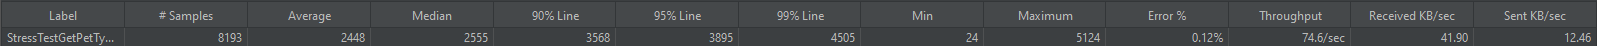
\includegraphics[width=\textwidth]{figs/Performance/Results/JMETER GET STRESS AR.png}
			\caption{GET Stress Test Aggregate Report}
			\label{fig:GETStressAggregateReport}
		\end{figure}
		\begin{figure}[H]
			\centering
			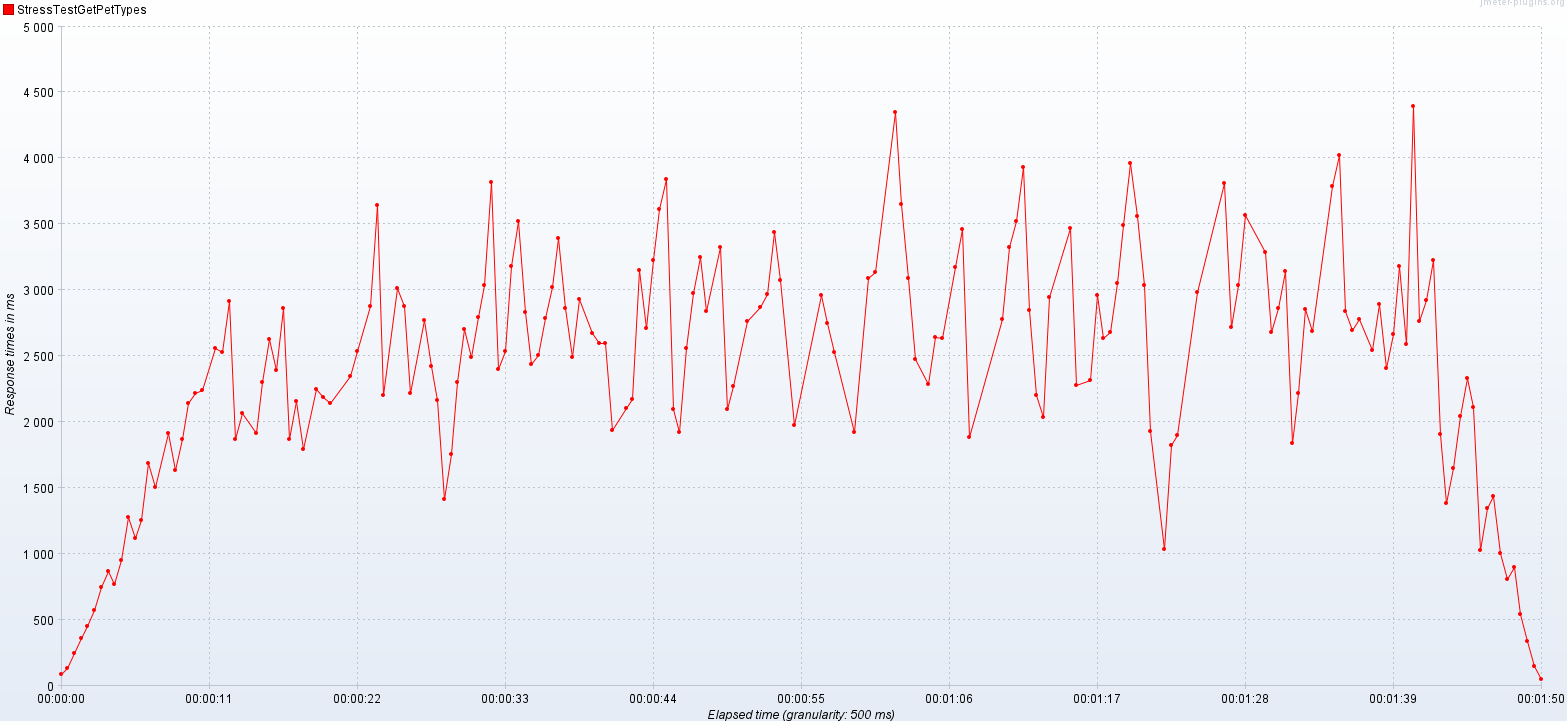
\includegraphics[width=0.7\textwidth]{figs/Performance/Results/JMETER GET STRESS ROT.png}
			\caption{GET Stress Test Responses Over Time}
			\label{fig:GETStressResposesOverTime}
		\end{figure}
		The results, seen in Figure \ref{fig:GETStressAggregateReport}, indicate that the API performs well under this scenario, with just 0.12\% errors and an average response time of 2448 ms. The highest response time was just 5124 ms, which is a little over the maximum defined, and therefore was counted as an error.
		In Figure \ref{fig:GETStressResposesOverTime}, we can see the response times over time, which, unlike the LoadTest, did not remain stable throughout the entire process	

		
		\subsection{K6}
		\textbf{Test Configuration}
		\begin{figure}[H]
			\centering
			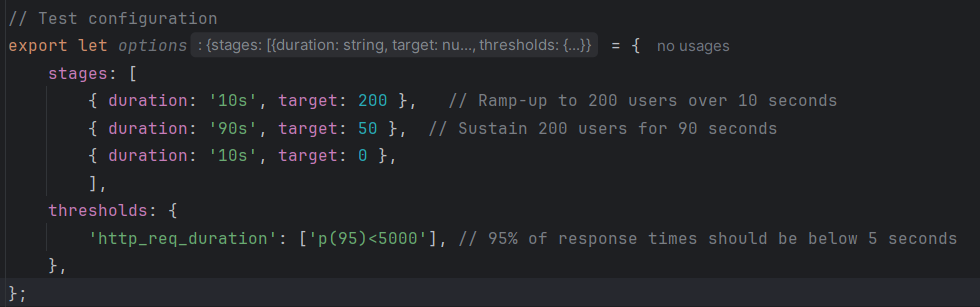
\includegraphics[width=0.7\textwidth]{figs/Performance/Test Configuration/K6-STRESS.png}
			\caption{K6 Stress Configuration}
			\label{fig:K6-STRESS}
		\end{figure}
		Similar to the JMeter configuration, in the k6 test, I configured the test to hold 200 users for 90 seconds, as shown in Figure \ref{fig:K6-STRESS}. I've also set the Duration to be less than 5000 milliseconds.


		
		
		\textbf{Results}
		\begin{figure}[H]
			\centering
			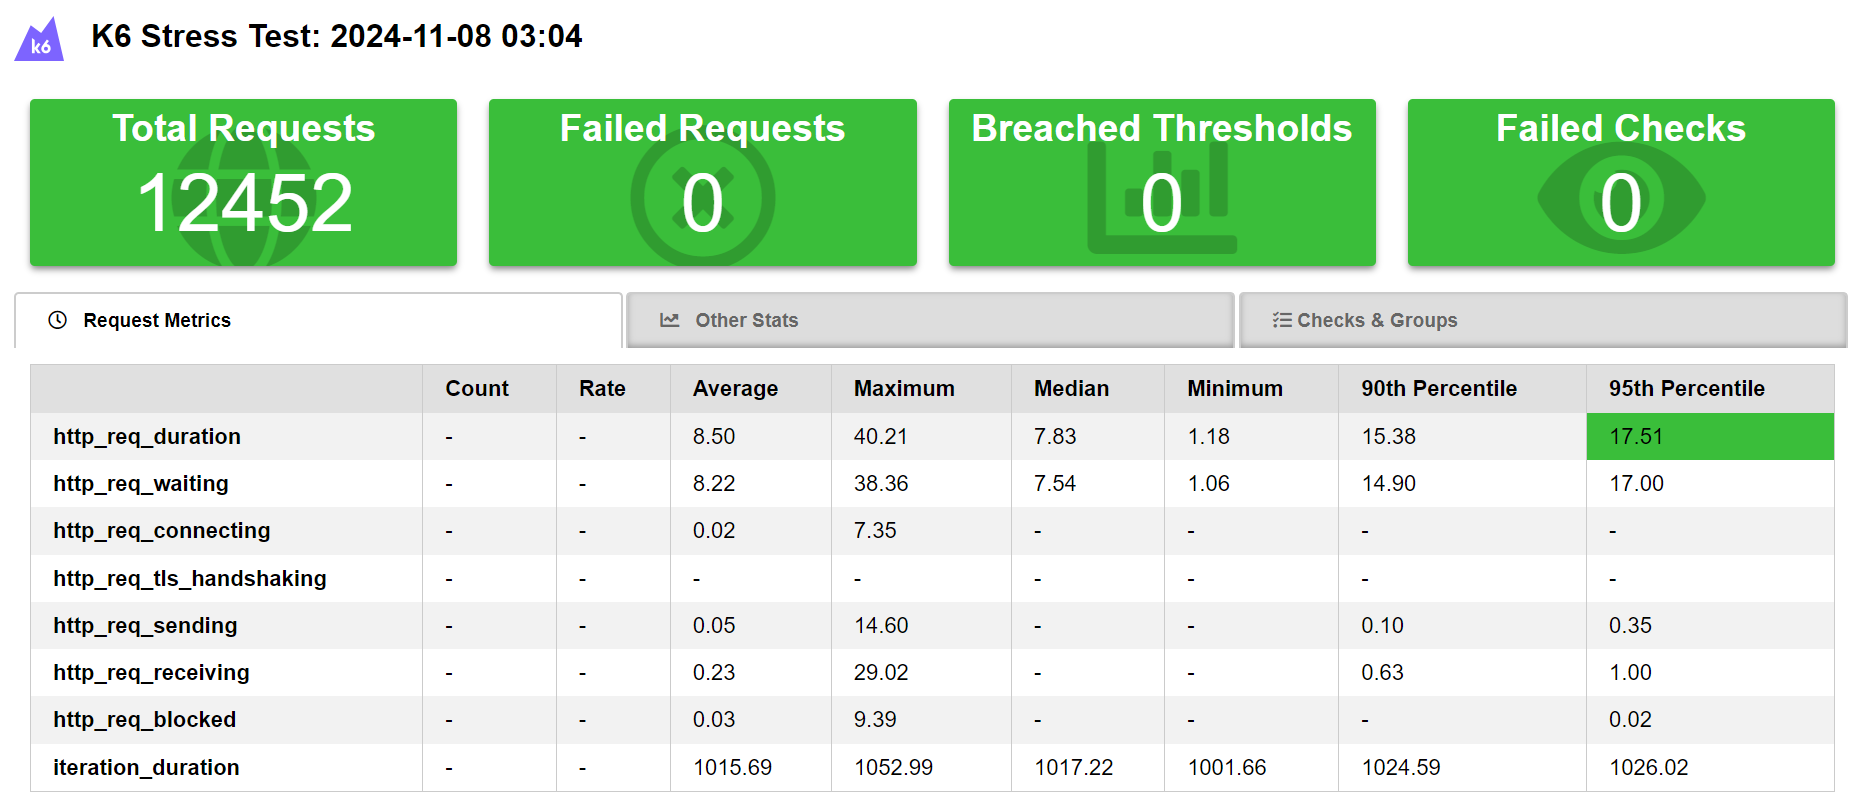
\includegraphics[width=0.7\textwidth]{figs/Performance/Results/K6 GET STRESS.png}
			\caption{K6 GET STRESS}
			\label{fig:K6-GET-STRESS}
		\end{figure}
		The results, seen in Figure \ref{fig:K6-GET-STRESS}, indicate that the API performs incredibly well under this scenario, with 0 failed request and an average response time of just 1015 ms. The highest response time was just 1052 ms, which is lower than the maximum defined.

		\subsection{Scenario POST}
		\begin{itemize}
			\item 200 users of the web application;
			\item Posting a new PetTypes
			\item The system returns 201
			\item Less than 5 seconds 95\% of the times;
			\item Heavy Load.
		\end{itemize}

		\subsection{Jmeter}
		\textbf{Test Configuration}
		\begin{figure}[H]
			\centering
			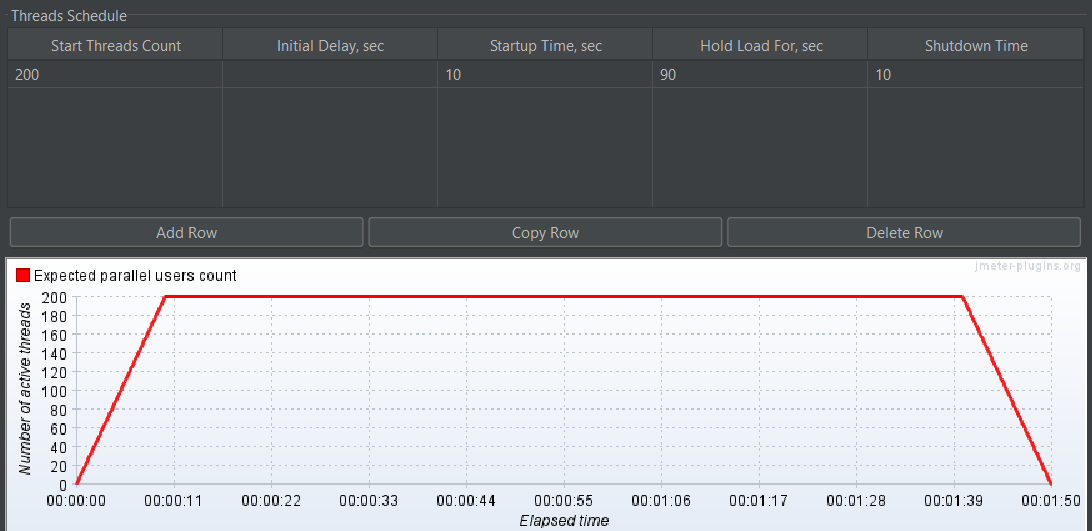
\includegraphics[width=0.7\textwidth]{figs/Performance/Test Configuration/JMETER-STRESS.png}
			\caption{Jmeter Stress Configuration}
			\label{fig:JMETER-STRESS-POST}
		\end{figure}
		\begin{figure}[H]
			\centering
			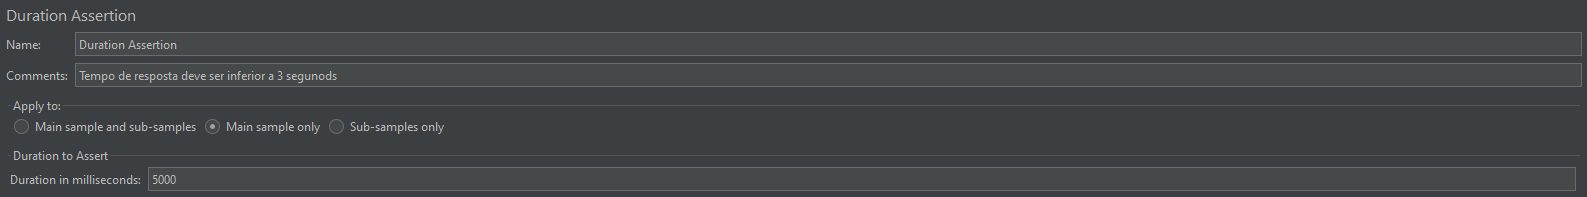
\includegraphics[width=0.7\textwidth]{figs/Performance/Test Configuration/Duration-Stress.png}
			\caption{Duration POST Stress Configuration}
			\label{fig:DurationPostStress}
		\end{figure}
		
		Based on the scenario we designed earlier I created the Jmeter Stress Configuration that holds for 90 seconds 200 Threads (Users), as seen in the Figure \ref{fig:JMETER-STRESS-POST}. In the Figure \ref{fig:DurationPostStress} I've set the maximum duration to 5000 milliseconds.

		
		\textbf{Results}
		\begin{figure}[H]
			\centering
			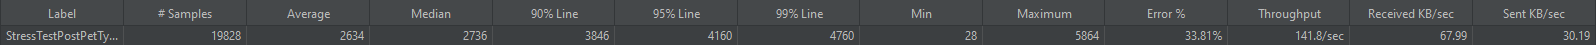
\includegraphics[width=\textwidth]{figs/Performance/Results/JMETER POST STRESS AR.png}
			\caption{POST Stress Test Aggregate Report}
			\label{fig:POSTStressAggregateReport}
		\end{figure}
		\begin{figure}[H]
			\centering
			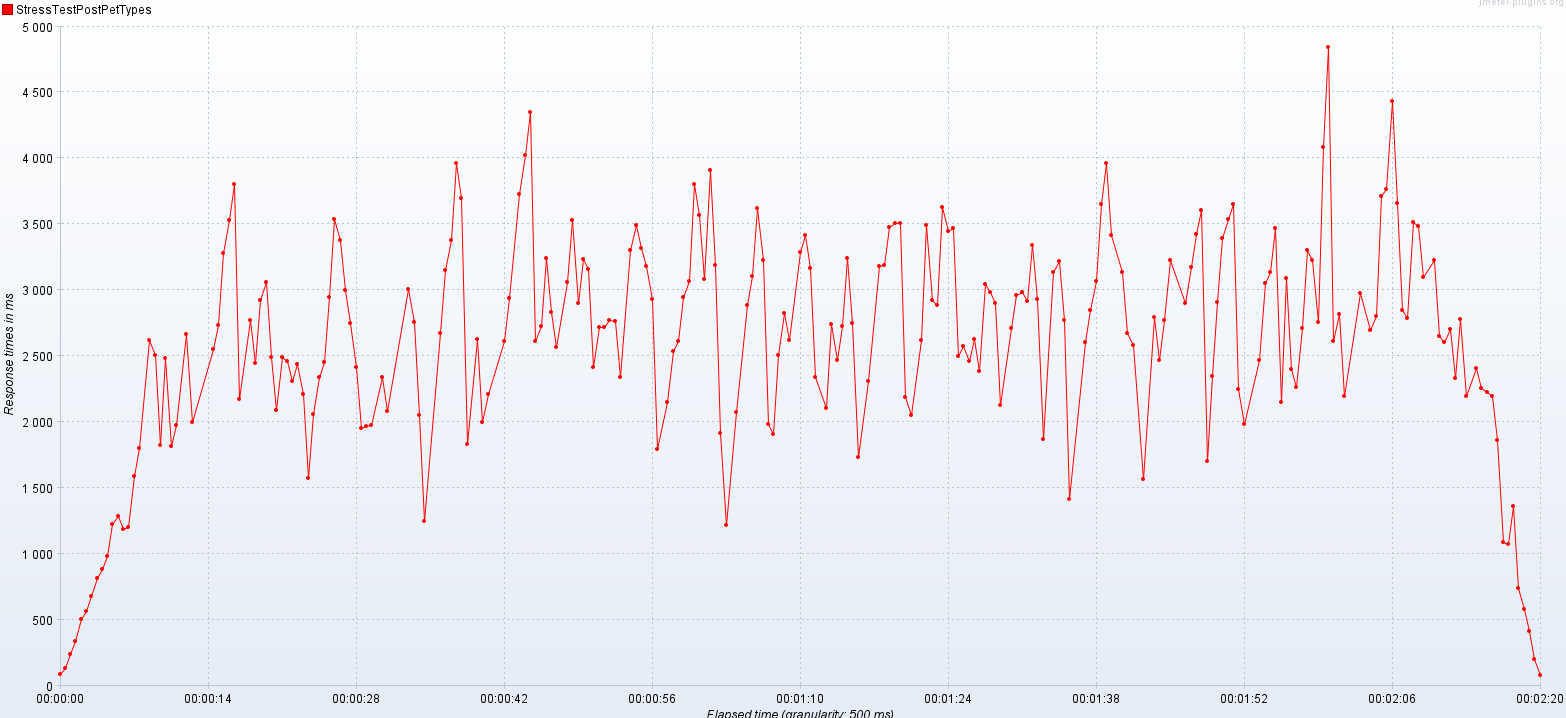
\includegraphics[width=0.7\textwidth]{figs/Performance/Results/JMETER POST STRESS ROT.png}
			\caption{POST Stress Test Responses Over Time}
			\label{fig:POSTStressResposesOverTime}
		\end{figure}

		The results, seen in Figure \ref{fig:POSTStressAggregateReport}, indicate that the API performs below the expected under this scenario, with 33.81\% errors and an average response time of 2634 ms. The highest response time was just 5864 ms, which is almost over a second higher than the maximum defined, and therefore was counted as an error.
		In Figure \ref{fig:POSTStressResposesOverTime}, we can see the response times over time, which, unlike the LoadTest, did not remain stable throughout the entire process	


		\subsection{K6}
		\textbf{Test Configuration}
		\begin{figure}[H]
			\centering
			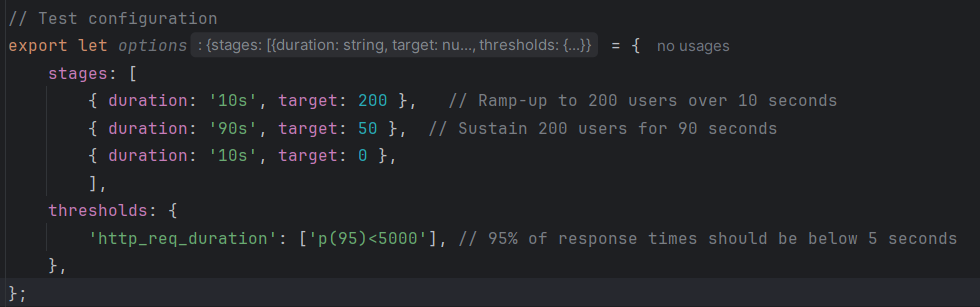
\includegraphics[width=0.7\textwidth]{figs/Performance/Test Configuration/K6-STRESS.png}
			\caption{K6 Stress Configuration}
			\label{fig:K6-STRESS-POST}
		\end{figure}
		Similar to the JMeter configuration, in the k6 test, I configured the test to hold 200 users for 90 seconds, as shown in Figure \ref{fig:K6-STRESS-POST}. I've also set the Duration to be less than 5000 milliseconds.
		
		
		\textbf{Results}

		\begin{figure}[H]
			\centering
			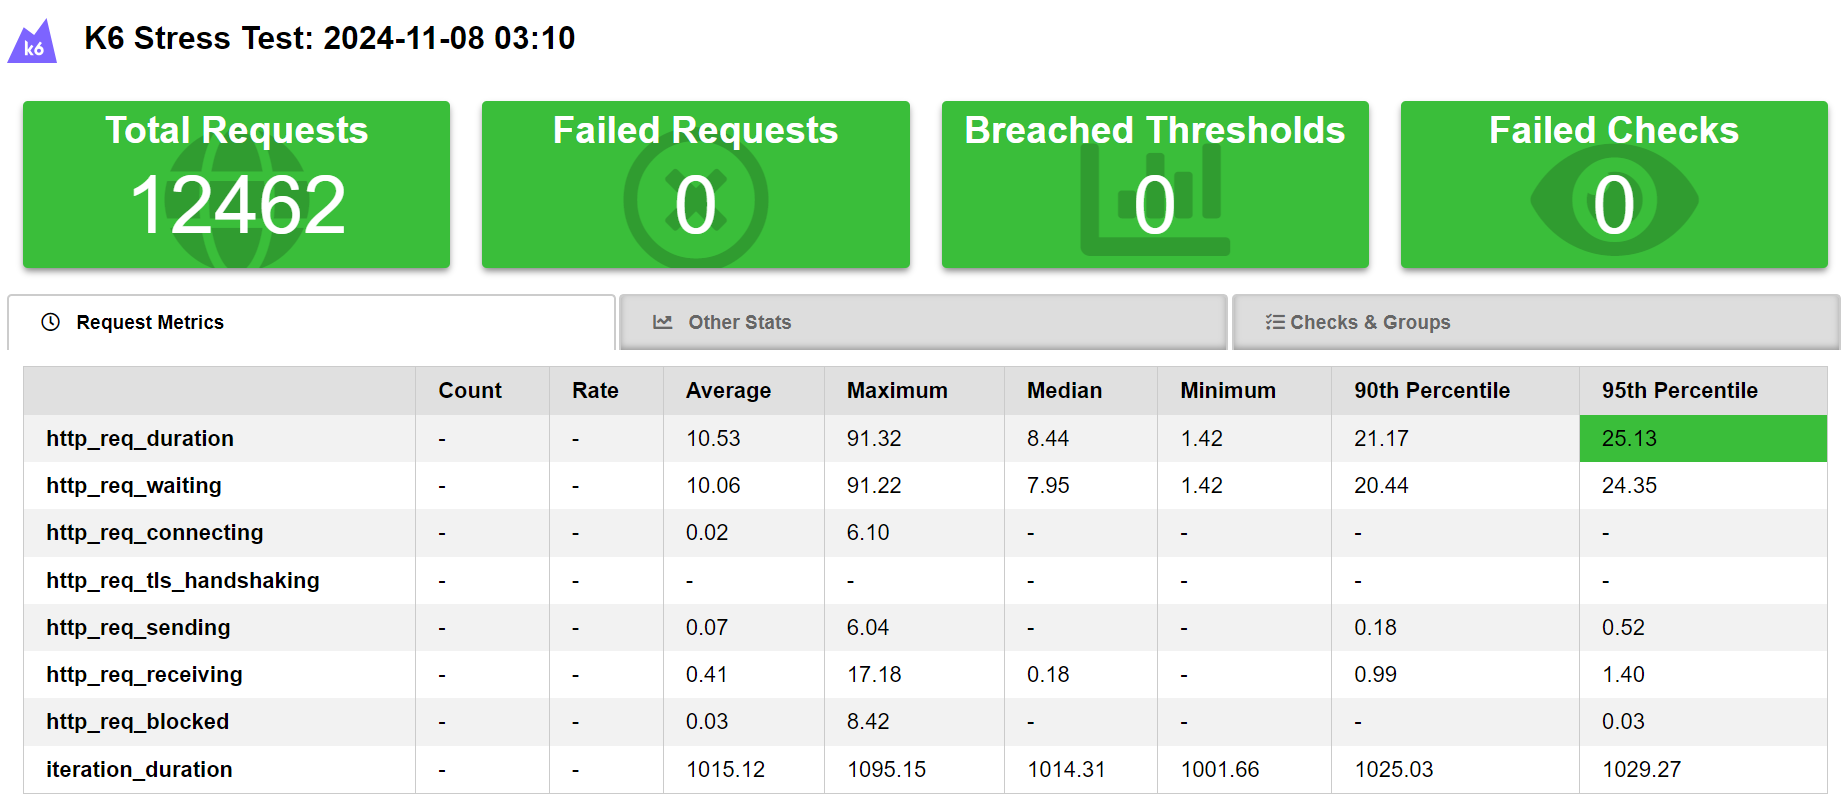
\includegraphics[width=0.7\textwidth]{figs/Performance/Results/K6 POST STRESS.png}
			\caption{K6 POST STRESS}
			\label{fig:K6-POST-STRESS}
		\end{figure}
		The results, seen in Figure \ref{fig:K6-POST-STRESS}, indicate that the API performs incredibly well under this scenario, with 0 failed request and an average response time of just 1015 ms. The highest response time was just 1095 ms, which is lower than the maximum defined.


\section{Soak Test}
		
Soak testing involves running a system at normal load levels for an extended period to identify performance issues that may not be apparent during shorter testing phases. This type of testing helps uncover problems such as memory leaks, resource depletion, and degradation in response times over time. By maintaining a steady load, soak tests provide insights into the system’s long-term reliability and stability, ensuring it can handle sustained usage without performance deterioration. In this section, we will evaluate the soak tests for the endpoints GET and POST of petType.		
		\subsection{Scenario GET}
		\begin{itemize}
			\item 50 users of the web application;
			\item Sending the petType information to the application;
			\item The application gives a success or error response to the user;
			\item Less than 5 seconds 95\% of the times;
			\item Normal Load.
		\end{itemize}

		\subsection{Jmeter}
		\textbf{Test Configuration}
		\begin{figure}[H]
			\centering
			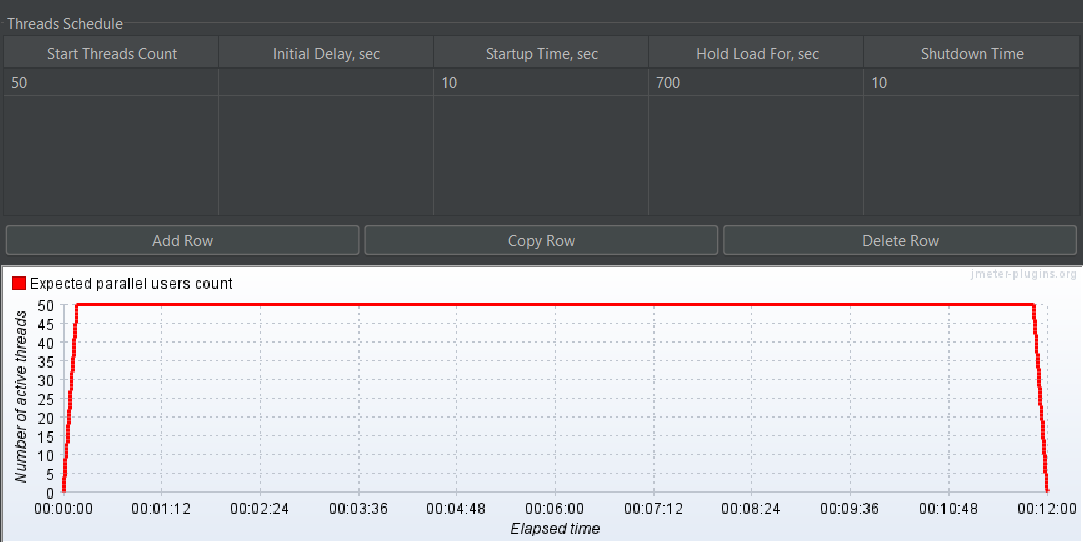
\includegraphics[width=0.7\textwidth]{figs/Performance/Test Configuration/JMETER-SOAK.png}
			\caption{Jmeter SOAK Configuration}
		 	\label{fig:JMETER-SOAK}
		\end{figure}
		\begin{figure}[H]
			\centering
			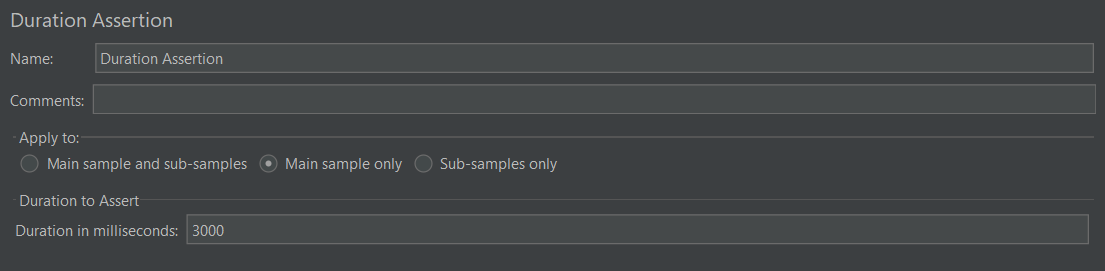
\includegraphics[width=0.7\textwidth]{figs/Performance/Test Configuration/Duration-SOAK-LOAD-JMETER.png}
			\caption{Duration GET Soak Configuration}
			\label{fig:DurationGetSoak}
		\end{figure}
		
		Based on the scenario we designed earlier I created the Jmeter Soak Configuration that holds for 700 seconds 50 Threads (Users), as seen in the Figure \ref{fig:JMETER-SOAK}. In the Figure \ref{fig:DurationGetSoak} I've set the maximum duration to 3000 milliseconds.

		\textbf{Results}
		
		\begin{figure}[H]
			\centering
			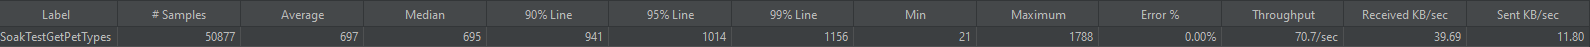
\includegraphics[width=\textwidth]{figs/Performance/Results/JMETER GET SOAK AR.png}
			\caption{GET Soak Test Aggregate Report}
			\label{fig:GETSoakAggregateReport}
		\end{figure}
		\begin{figure}[H]
			\centering
			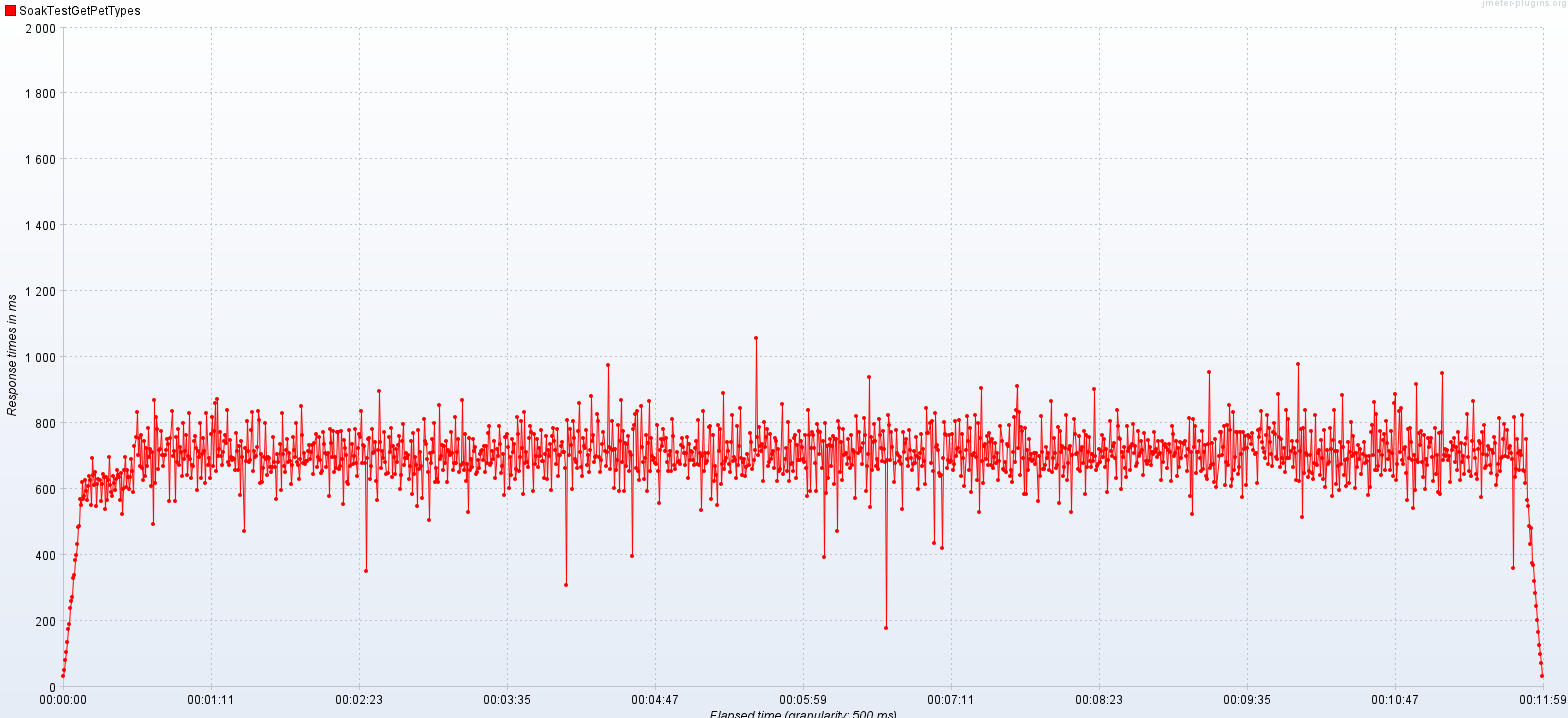
\includegraphics[width=0.7\textwidth]{figs/Performance/Results/JMETER GET SOAK ROT.png}
			\caption{GET Soak Test Responses Over Time}
			\label{fig:GETSoakResposesOverTime}
		\end{figure}
		
		The results, seen in Figure \ref{fig:GETSoakAggregateReport}, indicate that the API performs incredibly well under this scenario, with 0\% errors and an average response time of 679 ms. The highest response time was just 1788 ms, which equates a little over half of the maximum defined.
		In Figure \ref{fig:GETSoakResposesOverTime}, we can see the response times over time, which remained stable throughout the entire process.





		\subsection{K6}
		\textbf{Test Configuration}
		\begin{figure}[H]
			\centering
			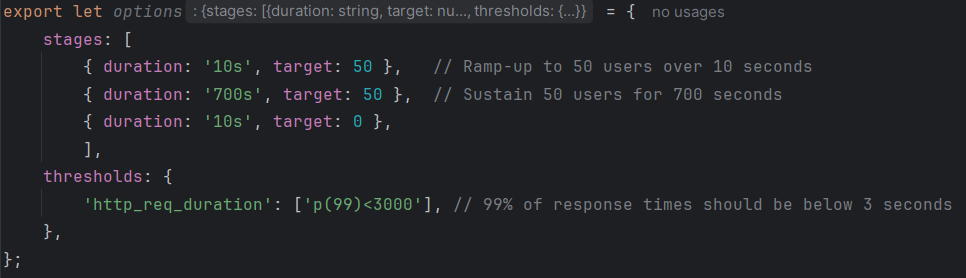
\includegraphics[width=0.7\textwidth]{figs/Performance/Test Configuration/K6-SOAK.png}
			\caption{K6 Soak Configuration}
			\label{fig:K6-Soak}
		\end{figure}
		Similar to the JMeter configuration, in the k6 test, I configured the test to hold 50 users for 700 seconds, as shown in Figure \ref{fig:K6-Soak}. I've also set the Duration to be less than 3000 milliseconds.


		\textbf{Results}
		\begin{figure}[H]
			\centering
			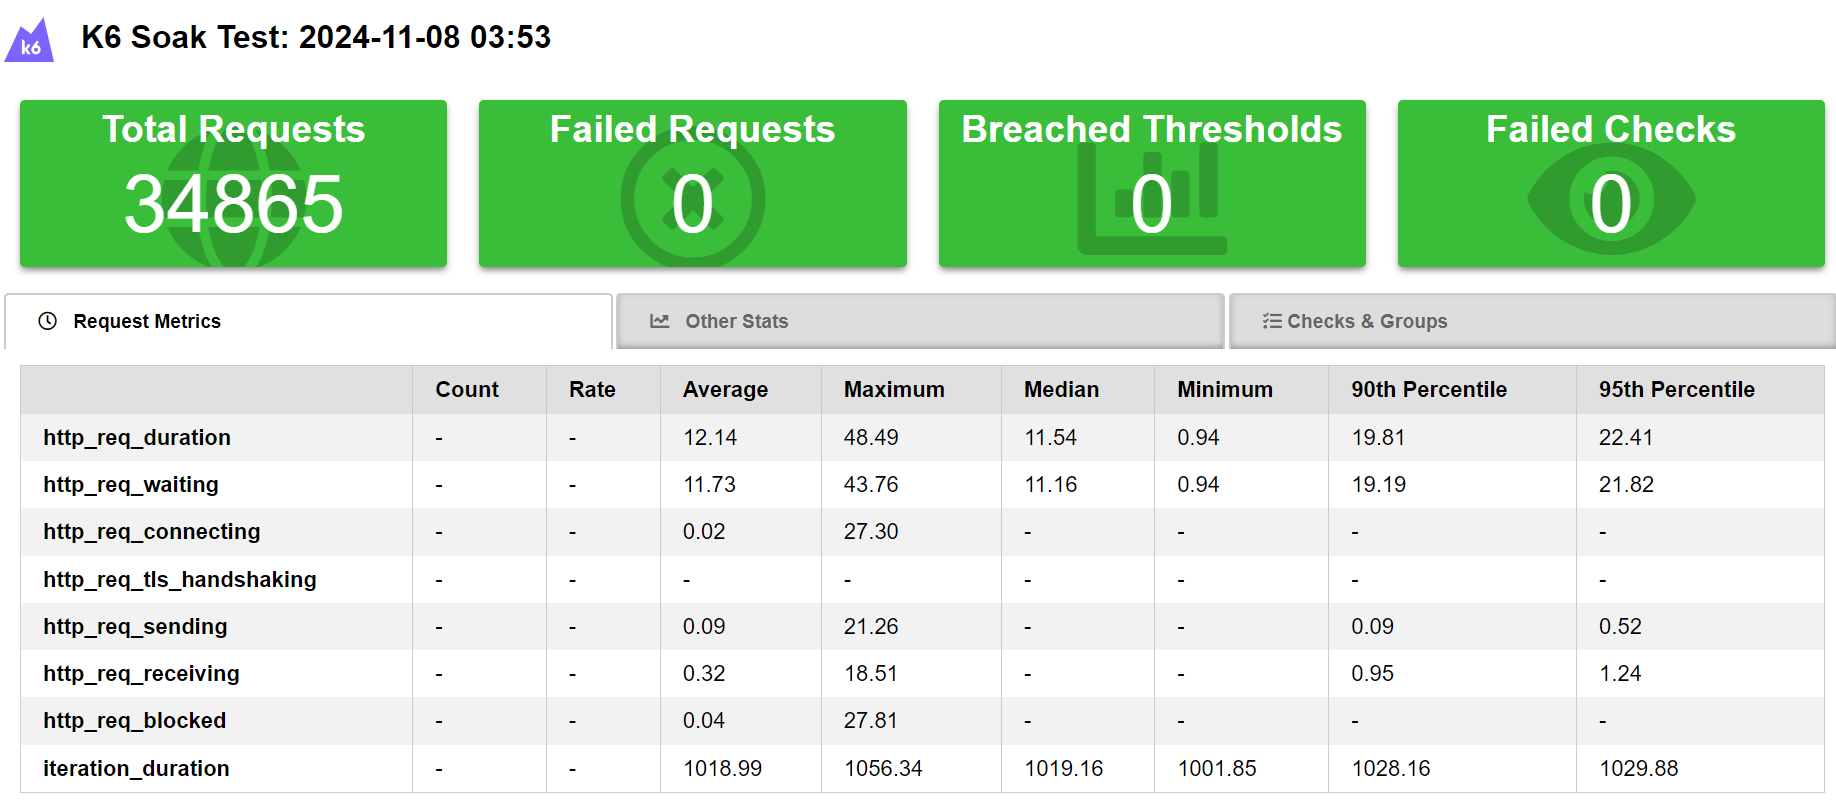
\includegraphics[width=0.7\textwidth]{figs/Performance/Results/K6 GET SOAK.png}
			\caption{K6 GET SOAK}
			\label{fig:K6-GET-SOAK}
		\end{figure}

		The results, seen in Figure \ref{fig:K6-GET-SOAK}, indicate that the API performs incredibly well under this scenario, with 0 failed request and an average response time of just 1018 ms. The highest response time was just 1056 ms, which is lower than the maximum defined.

		  \subsection{Scenario POST}
		  \begin{itemize}
			  \item 200 users of the web application;
			  \item Posting a new PetTypes
			  \item The system returns 201
			  \item Less than 5 seconds 95\% of the times;
			  \item Heavy Load.
		  \end{itemize}
  
		  \subsection{Jmeter}
		  \textbf{Test Configuration}
		\begin{figure}[H]
			  \centering
			  \includegraphics[width=0.7\textwidth]{figs/Performance/Test Configuration/JMETER-SOAK.png}
			  \caption{Jmeter Soak Configuration}
			  \label{fig:JMETER-Soak-POST}
		\end{figure}
		\begin{figure}[H]
			\centering
			\includegraphics[width=0.7\textwidth]{figs/Performance/Test Configuration/Duration-SOAK-LOAD-JMETER.png}
			\caption{Duration POST Soak Configuration}
			\label{fig:DurationPostSoak}
		\end{figure}
		Based on the scenario we designed earlier I created the Jmeter Soak Configuration that holds for 700 seconds 50 Threads (Users), as seen in the Figure \ref{fig:JMETER-Soak-POST}. In the Figure \ref{fig:DurationPostSoak} I've set the maximum duration to 3000 milliseconds.

		  
		  
		  \textbf{Results}

		  \begin{figure}[H]
			\centering
			\includegraphics[width=\textwidth]{figs/Performance/Results/JMETER POST SOAK AR.png}
			\caption{POST Soak Test Aggregate Report}
			\label{fig:POSTSoakAggregateReport}
		\end{figure}
		\begin{figure}[H]
			\centering
			\includegraphics[width=0.7\textwidth]{figs/Performance/Results/JMETER POST SOAK ROT.png}
			\caption{POST Soak Test Responses Over Time}
			\label{fig:POSTSoakResposesOverTime}
		\end{figure}

		The results, seen in Figure \ref{fig:POSTSoakAggregateReport}, indicate that the API performs incredibly well under this scenario, with 0\% errors and an average response time of 735 ms. The highest response time was just 2200 ms, which is lower than the maximum defined.
		In Figure \ref{fig:POSTSoakResposesOverTime}, we can see the response times over time, which remained stable throughout the entire process.


		  \subsection{K6}
		  \textbf{Test Configuration}
		\begin{figure}[H]
			\centering
			\includegraphics[width=0.7\textwidth]{figs/Performance/Test Configuration/K6-SOAK.png}
			\caption{K6 Soak Configuration}
			\label{fig:K6-Soak-POST}
		\end{figure}
		Similar to the JMeter configuration, in the k6 test, I configured the test to hold 50 users for 700 seconds, as shown in Figure \ref{fig:K6-Soak-POST}. I've also set the Duration to be less than 3000 milliseconds.

		\textbf{Results}
		\begin{figure}[H]
			\centering
			\includegraphics[width=0.7\textwidth]{figs/Performance/Results/K6 POST SOAK.png}
			\caption{K6 POST SOAK}
			\label{fig:K6-POST-SOAK}
		\end{figure}
		The results, seen in Figure \ref{fig:K6-POST-SOAK}, indicate that the API performs incredibly well under this scenario, with 0 failed request and an average response time of just 1015 ms. The highest response time was just 1053 ms, which is lower than the maximum defined.


		\section{Conclusion}

In conclusion, the application's performance was extremely good across most scenarios, with stable response times and minimal errors observed. The API consistently demonstrated low average response times and stayed well within the maximum limits in both load and soak tests. However, under the POST stress test, performance declined, showing a 33.81\% error rate and response times that exceeded the expected maximum threshold. This indicates that while the application is robust in general load conditions, improvements may be necessary to handle high-stress scenarios in POST requests.
 %% =================================
	\chapter{Security}
\textit{	In today's digital landscape, security has emerged as a paramount concern for both individuals and organizations, particularly as applications become more sophisticated and deeply embedded within critical infrastructure. The growing complexity of software systems increases the risk of security breaches, particularly through vulnerabilities in third-party dependencies that attackers may exploit to compromise data, disrupt operations, or gain unauthorized access.}
\section{Dependency Checker}
Based on the report generated by the OWASP Dependency Check plugin, the following dependencies were detected:
\begin{itemize}
	\item jackson-databind-2.15.3.jar
	\item mysql-connector-j-8.1.0.jar
	\item postgresql-42.6.0.jar
	\item spring-core-6.1.2.jar
	\item spring-security-core-6.2.1.jar
	\item spring-security-web-6.2.1.jar
	\item spring-webmvc-6.1.2.jar
\end{itemize}

Now, I will focus my analysis on the spring-core-6.1.2.jar dependency.

\section{Spring Core Dependency}
The spring-core-6.1.2 version had 2 Common Vulnerabilities and Exposure (CVE). The highest severity of those CVE is HIGH, which means that the problem 
\subsection{Identified Vulnerabilities}

\textbf{CVE-2024-22233}
\begin{itemize}
	\item \textbf{Description: }This vulnerability allows a user to send specially crafted HTTP requests that may cause a denial-of-service (DoS) condition.
	\item \textbf{Score: }7.5 \textbf{High} on the CVSSv3 scale
	\item \textbf{Solution:} The recommended solution is to update spring-core to version 6.1.14, where this vulnerability is patched, and configure the application to mitigate potential DoS issues.
\end{itemize}
\textbf{CVE-2024-38820}
\begin{itemize}
	\item \textbf{Description: }The fix for CVE-2022-22968 made disallowedFields patterns in DataBinder case insensitive. However, String.toLowerCase() has some Locale dependent exceptions that could potentially result in fields not protected as expected.
	\item \textbf{Impact Score: }5.3 \textbf{Medium} on the CVSSv3 scale
	\item \textbf{Solution:} An update to a version beyond 6.1.14 addresses this issue. Additionally, manual reviews of binding configurations can ensure safe data handling.
\end{itemize}

\subsection{CVSS3 Scale}
In order to better understand the Impact Scores I decided to show how the labels are attributed
\begin{itemize}
	\item \textbf{Critical:} 9.0 - 10
	\item \textbf{High:} 7.0 - 8.9
	\item \textbf{Medium:} 4.0 - 6.9
	\item \textbf{Low:} 0.1 - 3.9
\end{itemize}
%% =================================
	\chapter{Architectural compliance}
	This section focuses on assessing the architectural compliance of the application, ensuring it aligns with the defined guidelines. Using ArchUnit, we create fitness functions to detect architectural issues like package dependencies, class dependencies, inheritance misuse, and layer violations. We will specifically examine the petType Aggregate to verify adherence to these standards. The goal is to identify and correct any deviations, ensuring the application remains scalable, maintainable, and efficient.

	\section{Package Dependency}
	\subsection{Code}
	\begin{figure}[H]
		\centering
		\includegraphics[width=0.7\textwidth]{figs/Architectural Compliance/Package Dependency Code.png}
		\caption{Package Dependency Code}
		\label{fig:Class-Dependency-Code}
	\end{figure}

	This test ensures that the PetType class in the model package does not depend on classes from the controller, repository, or dto packages.
	\subsection{Result}
	\begin{figure}[H]
		\centering
		\includegraphics[width=0.7\textwidth]{figs/Architectural Compliance/PackageDependency.png}
		\caption{Package Dependency Test Result}
		\label{fig:Package-Dependency}
	\end{figure}
	As shown in the Figure \ref{fig:Package-Dependency}, the test was successful.
	
	
	
	
	
	\section{Class Dependency}
	\subsection{Code}
	\begin{figure}[H]
		\centering
		\includegraphics[width=0.7\textwidth]{figs/Architectural Compliance/Class Dependency Code.png}
		\caption{Class Dependency Code}
		\label{fig:Class-Dependency-Code}
	\end{figure}
	
This test ensures that classes with "PetType" in their name can only have dependencies on other classes with "PetType" in their name.
	\subsection{Result}
	\begin{figure}[H]
		\centering
		\includegraphics[width=0.7\textwidth]{figs/Architectural Compliance/Class Dependency.png}
		\caption{Class Dependency Test Result}
		\label{fig:Class-Dependency}
	\end{figure}
	
	As shown in the Figure \ref{fig:Class-Dependency}, the test has failed. It was violated 53 times.
	
	
	
	\section{Class and Package Containment}
	\subsection{Code}
	\begin{figure}[H]
		\centering
		\includegraphics[width=0.7\textwidth]{figs/Architectural Compliance/Class and Package Code.png}
		\caption{Class and Package Containment Code}
		\label{fig:Class-and-Package-Containment-Code}
	\end{figure}
	This test checks if specific classes like PetTypeRestController, PetTypeRepository, and others reside in their correct packages (rest.controller, repository, repository.jpa, rest.dto).
	\subsection{Result}
	\begin{figure}[H]
		\centering
		\includegraphics[width=0.7\textwidth]{figs/Architectural Compliance/Class and Package Containment.png}
		\caption{Class and Package Containment Test Result}
		\label{fig:Class-and-Package-Containment}
	\end{figure}
	As shown in the Figure \ref{fig:Class-and-Package-Containment}, the test was successful.

	
	
	
	
	\section{Inheritance}
	\subsection{Code}
	\begin{figure}[H]
		\centering
		\includegraphics[width=0.7\textwidth]{figs/Architectural Compliance/Inhritance Code.png}
		\caption{Inheritance Code}
		\label{fig:Inheritance-Code}
	\end{figure}
	The first test ensures that JpaPetTypeRepository implements PetTypeRepository. The second test ensures that PetType inherits from itself.
	\subsection{Result}
	\begin{figure}[H]
		\centering
		\includegraphics[width=0.7\textwidth]{figs/Architectural Compliance/Inheritance.png}
		\caption{Inheritance Test Result 1}
		\label{fig:Inheritance-1}
	\end{figure}
	\begin{figure}[H]
		\centering
		\includegraphics[width=0.7\textwidth]{figs/Architectural Compliance/Inheritance2.png}
		\caption{Inheritance Test Result 1}
		\label{fig:Inheritance-2}
	\end{figure}
	As shown in the Figure \ref{fig:Inheritance-1} and Figure \ref{Inheritance-2}, both tests were successful.







	\section{Annotation}
	\subsection{Code}
	\begin{figure}[H]
		\centering
		\includegraphics[width=0.7\textwidth]{figs/Architectural Compliance/AnnotationCode.png}
		\caption{Annotation Code}
		\label{fig:Annotation-Code}
	\end{figure}
	This test ensures that the PetTypeRestController class is annotated with RestController.
	\subsection{Result}		
	\begin{figure}[H]
		\centering
		\includegraphics[width=0.7\textwidth]{figs/Architectural Compliance/Annotation.png}
		\caption{Annotation Test Result}
		\label{fig:Annotation}
	\end{figure}
	As shown in the Figure \ref{fig:Annotation}, the test was successful.




	\section{Layer}
	\subsection{Code}
	\begin{figure}[H]
		\centering
		\includegraphics[width=0.7\textwidth]{figs/Architectural Compliance/Layer Code.png}
		\caption{Layer Code}
		\label{fig:Layer-Code}
	\end{figure}
	This test verifies that the architecture follows specific rules, where layers like "Controller" can only access "DTO", "Repository", and "Model", but not "Model" can access any layer, ensuring clean separation.
	\subsection{Result}
	\begin{figure}[H]
		\centering
		\includegraphics[width=0.7\textwidth]{figs/Architectural Compliance/Layer.png}
		\caption{Layer Test Result}
		\label{fig:Layer}
	\end{figure}
	As shown in the Figure \ref{fig:Layer}, the test was successful.




	\section{Cycle}
	\subsection{Code}
	\begin{figure}[H]
		\centering
		\includegraphics[width=0.7\textwidth]{figs/Architectural Compliance/Cycle Code.png}
		\caption{Cycle}
		\label{fig:Cycle-Code}
	\end{figure}
	This test ensures that there are no cyclic dependencies between the classes in the project.
	\subsection{Result}
	\begin{figure}[H]
		\centering
		\includegraphics[width=0.7\textwidth]{figs/Architectural Compliance/Cycle.png}
		\caption{Cycle Test Result}
		\label{fig:Cycle}
	\end{figure}
	As shown in the Figure \ref{fig:Cycle}, the test was successful.


	\section{Conclusion}
	In conclusion, the architectural compliance analysis confirms that the application largely adheres to the defined standards. Most tests on package dependencies, class containment, inheritance, annotations, and layer separation were successful, ensuring a well-structured and modular design. However, the Class Dependency test revealed some violations, suggesting areas for improvement in maintaining clear dependency boundaries. Addressing these issues will further enhance the system’s scalability and maintainability.
	%% =================================

	
	


	%% =================================
	\chapter{Conclusions }
	This project was focused on evaluating key aspects of the application, mostly the PetType aggregate. By addressing topics like Funcional Correctness, Maintainability, Performance, Security and Architectural Compliance, and based on the results, I can confidently conclude that the aggregate performed to the expected levels in nearly every aspect tested, indicating a well-functioning and robust design. 
	
	
	The development of this project allowed me to use and test different tools, which led to multiple challenges but undoubtedly provided a good opportunity to learn and improve my skills in software analysis and testing.




 





	
	\bibliographystyle{ACM-Reference-Format}
	\renewcommand\bibname{References}
	\bibliography{ref}
	\label{references}
	\addcontentsline{toc}{chapter}{References}
	
\end{document}